\documentclass[12pt, letterpaper]{article}
\usepackage[utf8]{inputenc}
\usepackage{graphicx}
\usepackage{amsmath}
\usepackage{placeins}
\makeatletter
\AtBeginDocument{%
  \expandafter\renewcommand\expandafter\subsection\expandafter
    {\expandafter\@fb@secFB\subsection}%
  \newcommand\@fb@secFB{\FloatBarrier
    \gdef\@fb@afterHHook{\@fb@topbarrier \gdef\@fb@afterHHook{}}}%
  \g@addto@macro\@afterheading{\@fb@afterHHook}%
  \gdef\@fb@afterHHook{}%
}
\makeatother
\makeatletter
\AtBeginDocument{%
  \expandafter\renewcommand\expandafter\subsection\expandafter{%
    \expandafter\@fb@secFB\subsection
  }%
}
\makeatother

\title{Ecology Counts!}
\author{Odalys Barrientos, Brianna Cirillo, Veronia Marquez}
\date{22 December 2020}

\begin{document}
\maketitle

\section{Statistical Methodology}
In this analysis, contingency tables were used to asses how many journal entries came from each of the independent variables used. A contingency table, which can also be called a cross tabulation, is a table that shows the frequency distribution of each of the variables. Data cleaning was performed, thus removing any data where the independent variable being looked at was not applicable. Therefore, we separated the data by continent, country, region, state, and ecosystem. We looked at each of these tables to determine if the number of journal entries in each category, of these variables, were equal or close in frequency. 

In order to better understand the distribution of the number of journal entries in each category, pie charts and bar graphs were made. This gave a visual representation of the distribution of journal entries in each independent variable. Therefore allowing for a visual analysis based on graphs and tables made.

To further analyze these categories, chi square tests were used to determine whether or not the observed amount of journal entries for each of the independent variables were equal. The Pearson's chi-squared test is used to determine whether there is a statistically significant difference between the expected frequencies and the observed frequencies in one or more categories of a contingency table. An assumption of the test is that observations are mutually exclusive and independent. Therefore, data cleaning was done to ensure this condition was met. But the data was not randomly sampled, which goes against one of the assumptions. Thus, the p-values obtained do not have any relevance or any real meaning in relation to the data.

Being that the data consists of predominantly categorical variables, some additional data was added. Square mileage of continent, country, region, and state were researched, in order to better estimate the expected number of journal entries in each category.This allowed for chi square tests to be run with expected frequencies, that match the square mileage of each of the independent variables. This allowed for more accurate expected frequencies of journal entries from each independent variable. Data cleaning was done to remove rows that did not contain applicable data for each independent variable. The assumption of random sampling is still violated, therefore the p-values obtained could not be used to draw conclusions.

\section{Results}
\subsection{Continent}
The continent category demonstrated if any or the amount of published articles completed their study in a particular continent. This allowed us to see which continent were more or less commonly seen for ecology work. The following contingency table counts the number of times a continent was represented in the data set.
\begin{table}[h]
\begin{center}
\begin{tabular}{|c|c|}
\textbf{Continent} & \textbf{Count}\\
$Africa$ & 5\\
$Asia$ &  14\\
$Australia$ &  2\\
$Europe$ & 34\\
$North America$ & 94\\
$South America$ & 13\\
$Oceania$ & 5\\
\end{tabular}
\end{center}
\caption{This is the contingency table for the continents. It shows the number of journal articles that had work done on each continent.}
\label{fig: Continent Contingency Table}
\end{table}
From the table above notice the number of published articles is higher in North America in comparison to the other continents.

If there is an assumption that the probability of each continent being represented in a journal entry is the same, then there should be the same number of counts for each continent. Below, is a XChi-Square test that shows if this statement is true or not. 

\begin{figure}[h]
\begin{center}
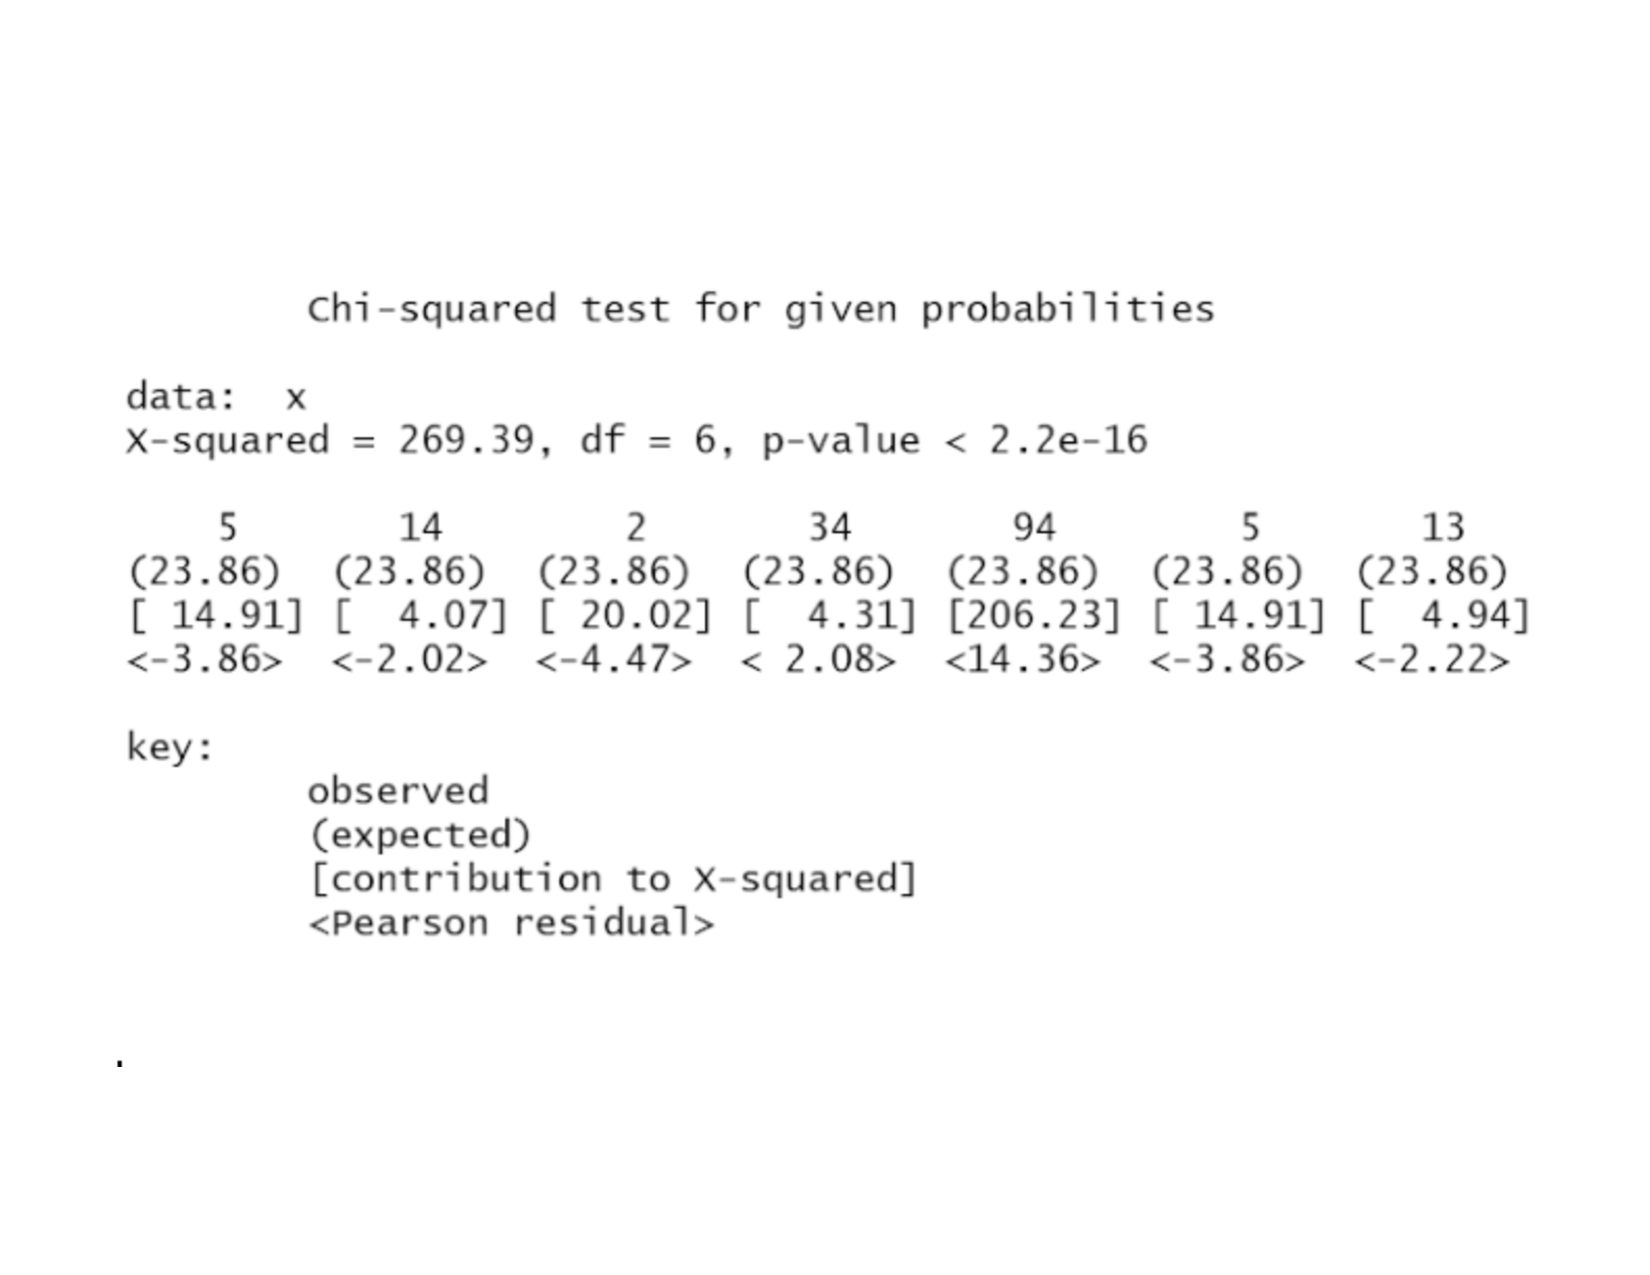
\includegraphics[width=10cm]{ContinentChiSqaure1.pdf}
\label{fig: Continent XChi-Square}
\caption{This is the XChi-Square test for the continents.}
\end{center}
\end{figure}

From the Pearson residuals notice that North America has the most positive residual thus, the observed frequency exceeds the expected frequency. Additionally, Australia has the most negative residual thus, the observed frequency does not meet the expected frequency. Through visual representation, figure *#* clarifies this idea. The pie chart on the left shows what the pie chart should look like if every continent had an equal chance of being represented in a published article. While the pie chart on the right is what the pie chart looks like when using the counts from the data set. 
\begin{figure}[h]
\begin{center}
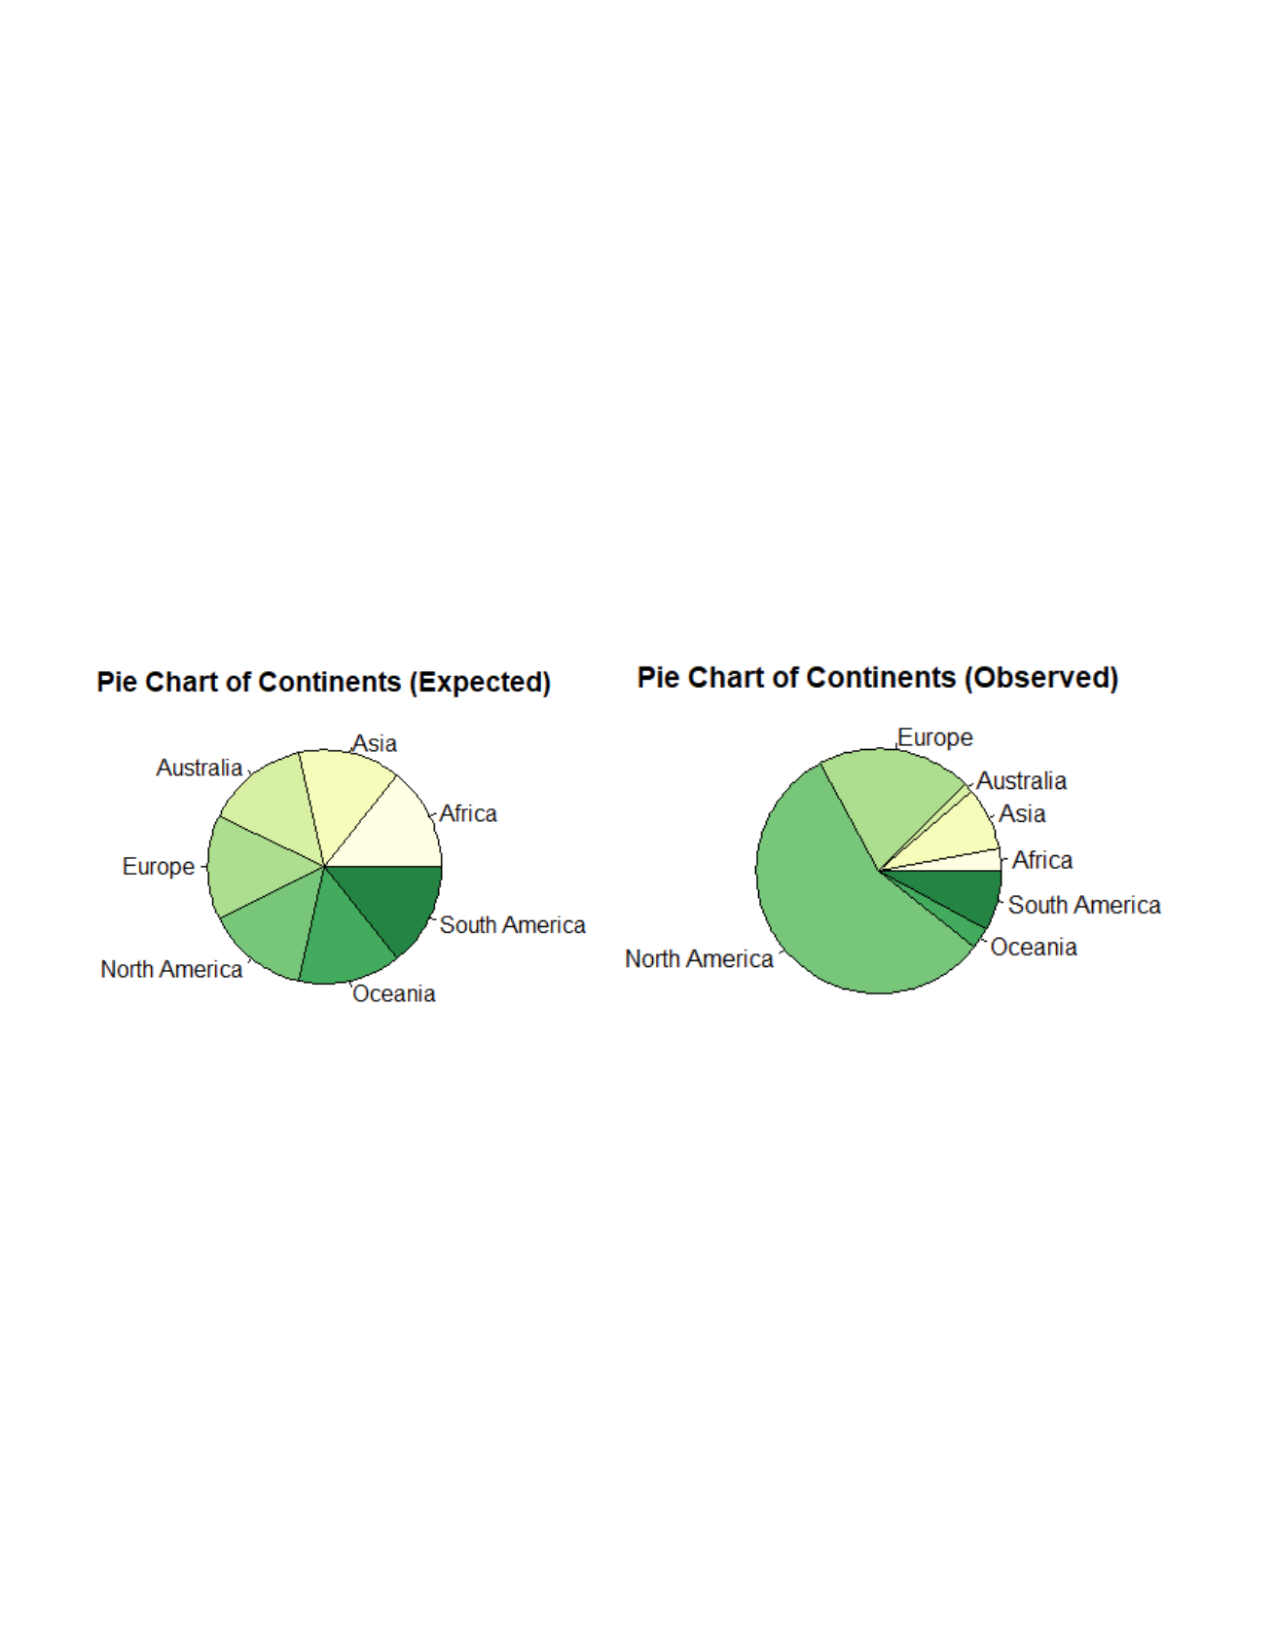
\includegraphics[width=10cm]{ContinentPieChart.pdf}
\label{fig: Continent Pie Chart}
\caption{This is a comparison of what the expected values for continent and the actual values for continent look like as pie charts.}
\end{center}
\end{figure}

If the continents had a equal chance of being represented in these published articles these pie charts would look similar. Unfortunately, this is not the case and it is obvious that North America takes up the majority of the pie chart.

If there is an assumption that the probability of each continent being represented in a journal entry is the same as each continent's square mileage. Then the continent with larger square mileage would have more published articles than those continent with a smaller square mileage. Below, is a XChi-Square test that shows if this statement is true or not.
 
\begin{figure}[h]
\begin{center}
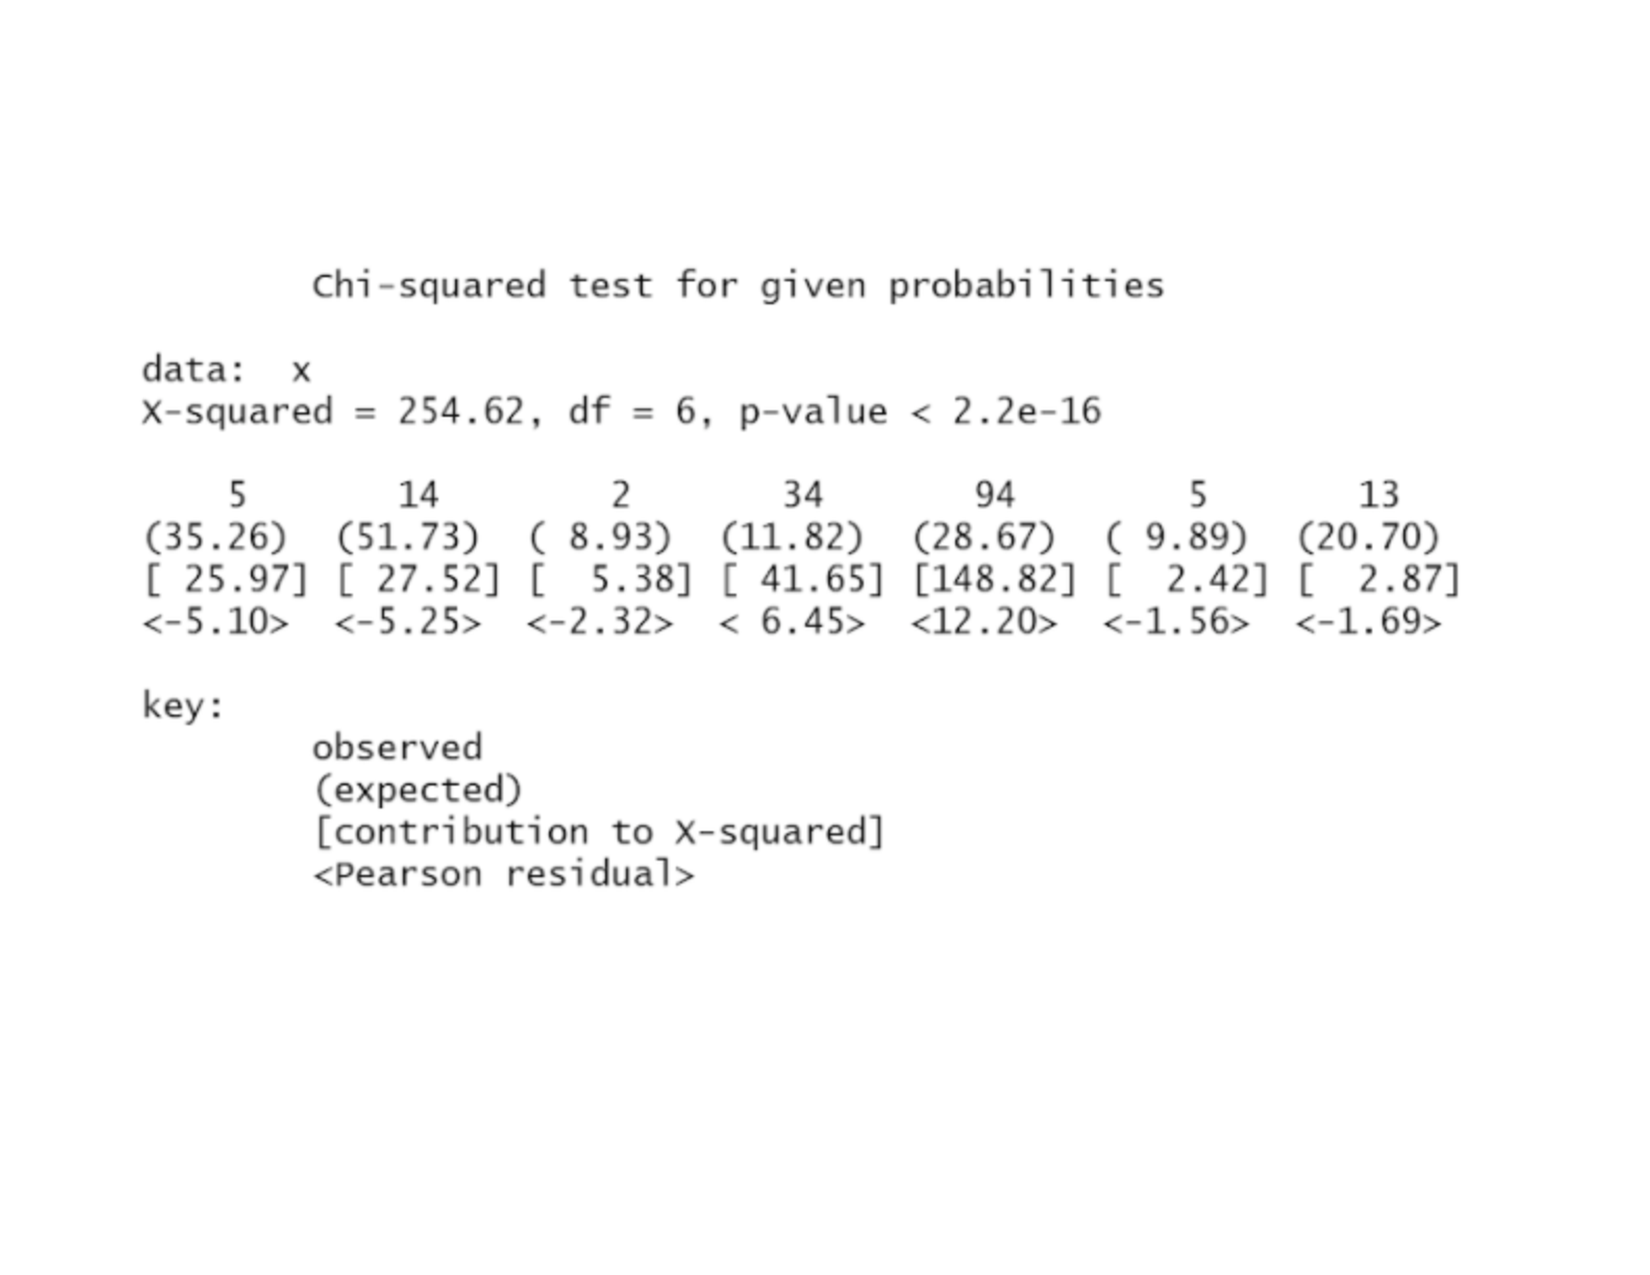
\includegraphics[width=10cm]{ContinentChiSquare2.pdf}
\label{fig: Continent XChi-Square with Square Mileage}
\caption{This is the XChi-Square test for the continents, using the square mileage data.}
\end{center}
\end{figure}

Looking into the Pearson residuals notice that North America has the most positive residual thus showing that the observed frequency exceeds the expected frequency. Through visual representation, figure *#* clarifies this idea. The bar graph on the left is the number of journals one expects to see given each continent's square mileage. The bar graph on the right is what was observed using the counts from the data set.
\begin{figure}[h]
\begin{center}
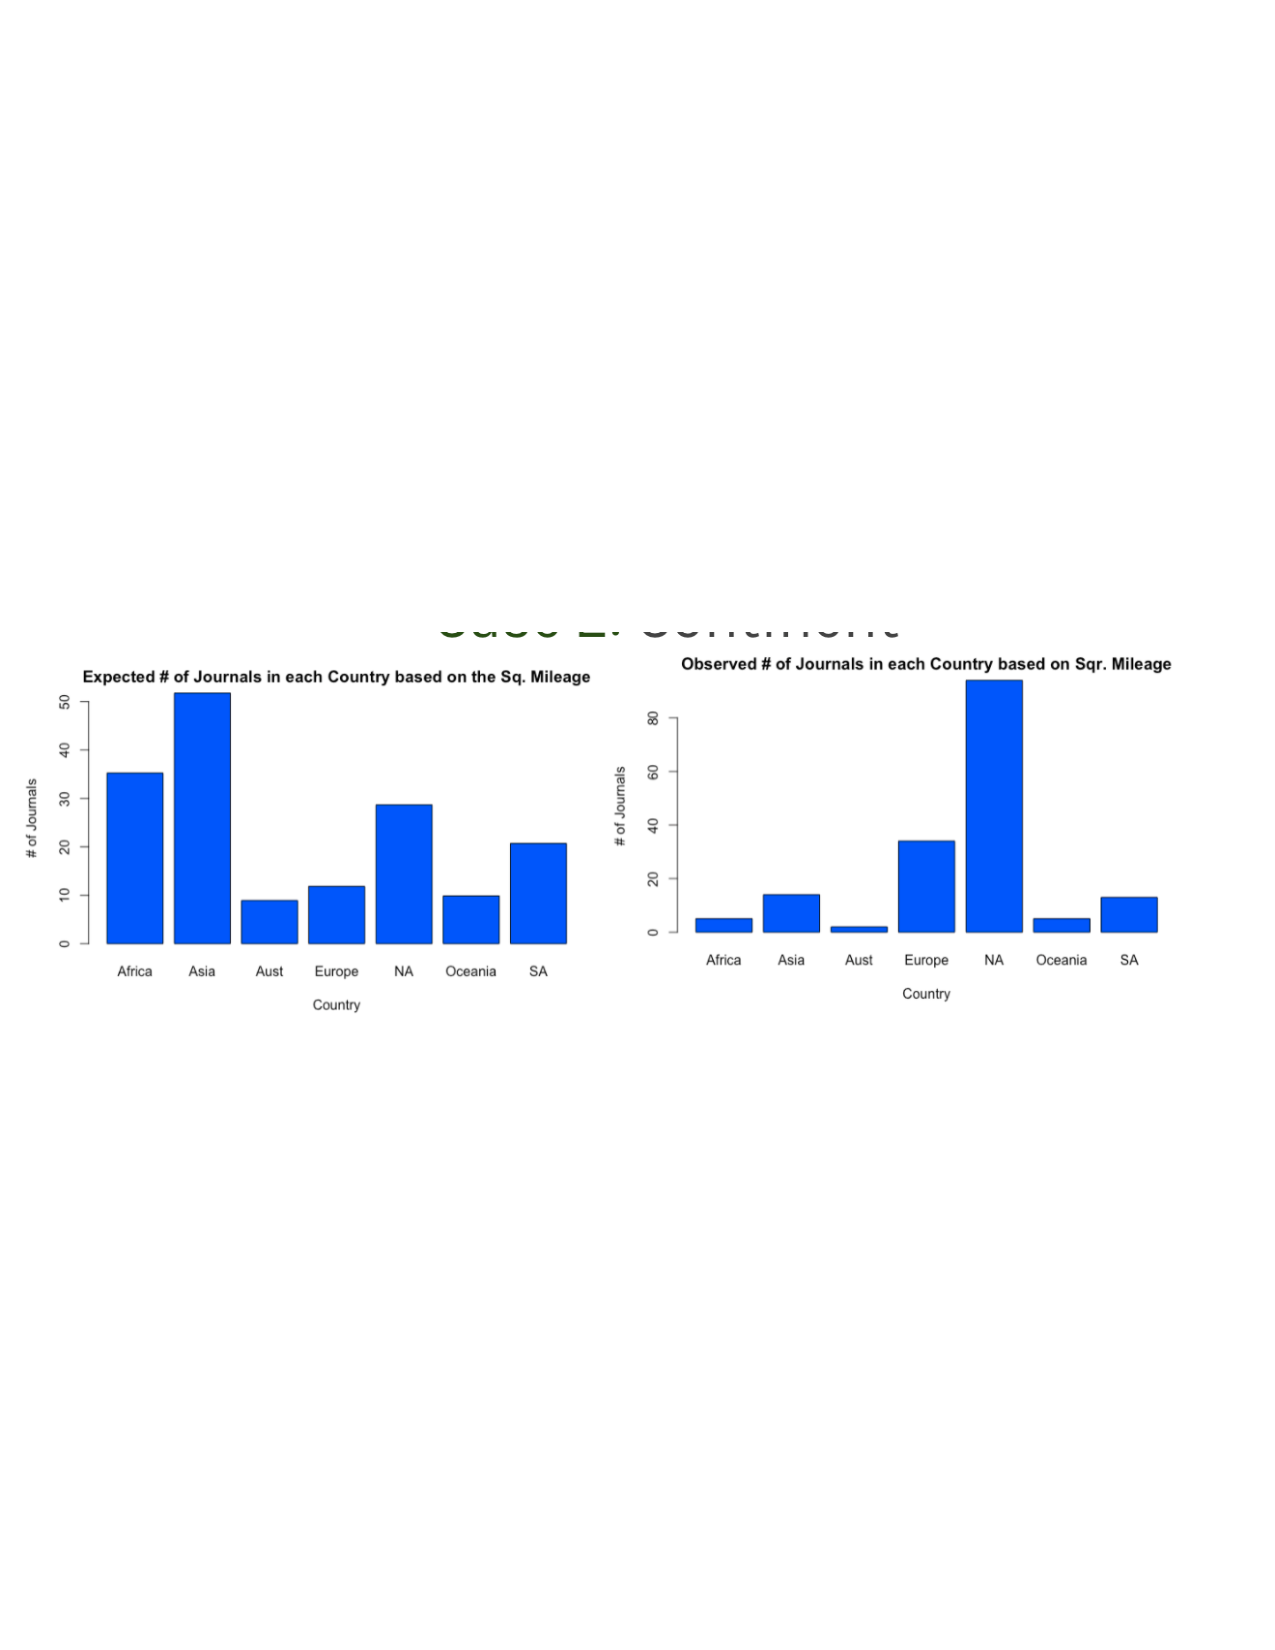
\includegraphics[width=0.10]{Continent2BarGraph.pdf}
\label{fig: Continent Bar Graph}
\caption{This is a bar graph comparing the expected and actual values for continent based on square mileage.}
\end{center}
\end{figure}

Asia is the continent with the largest square mileage in comparison to the other continents, and it has the largest number of expected journals based on it's square mileage. However it resulted in being one of the continent with the least number of journals based on the observed data. Asia and every continent besides North America never met the assumption. From the bar graph one can conclude that the probability of each continent being represented in a journal entry is not the same as the continents square mileage. In other words, giving that a continent is larger does not mean there are more published articles from that particular continent.

\pagebreak

\subsection{Country}
The variable country accounted for how many of these published articles completed the work done for the study in a particular country. Thus, we can see how many published articles from this collection of data have ecology work done in countries. To better model this, a contingency table was made to depict how frequently work done in a particular country was represented in the data set.
\begin{table}[h]
\begin{center}
\begin{tabular}{|c|c|}
\textbf{Country} & \textbf{Count}\\
$Argentina$ & 2\\
$Australia$ & 4\\
$Belgium$ & 1\\
$Bermuda$ & 1\\
$Brazil$ & 2\\
$Cambodia$ & 1\\
$Canada$ & 5\\
$China$ & 12\\
$Colombia$ & 2\\
$Costa Rica$ & 3\\
$England$ & 1\\
$Finland$ & 2\\
$France$ & 2\\
$French Guiana$ & 1\\
$Galapagos$ & 1\\
$Germany$ &  5\\
$Greece$ &  1\\
$Italy$ & 1\\
$Kenya$ & 2\\
$Mexico$ & 3\\
$New Zealand$ & 2\\
$Panama$ & 9\\
$Papua New Guinea$ &  1\\
$Peru$ &  2\\
$Portugal$ & 1\\
$Puerto Rico$ & 2\\
$Republic of Congo$ & 1\\
$Singapore$ & 1\\
$South Africa$ & 2\\
$Spain$ &  5\\
$St. John$ &  1\\
$Svalbard$ & 1\\
$Sweden$ & 5\\
$Switzerland$ & 4\\
$The Netherlands$ & 4\\
$USA$ & 68\\
\end{tabular}
\end{center}
\caption{This contingency table shows the frequency of countries in journal articles. Not all countries are represented because there were not journal articles that had work done in every country in the data set.}
\label{fig: Contingency Table for Country}
\end{table}

From the figure above, an be seen that the country where the study was done, that had the highest frequency of articles was the United States. There were 68 journal articles where the work was in the United States. This is different from the number of articles with work done in other countries, it was more common that each only had one or two journal articles. 

Using a chi squared test, we analyzed whether the probability of each country being represented in a journal article is the same. This test was run with the assumption that every country had an equal chance.

\begin{figure}[h]
\begin{center}
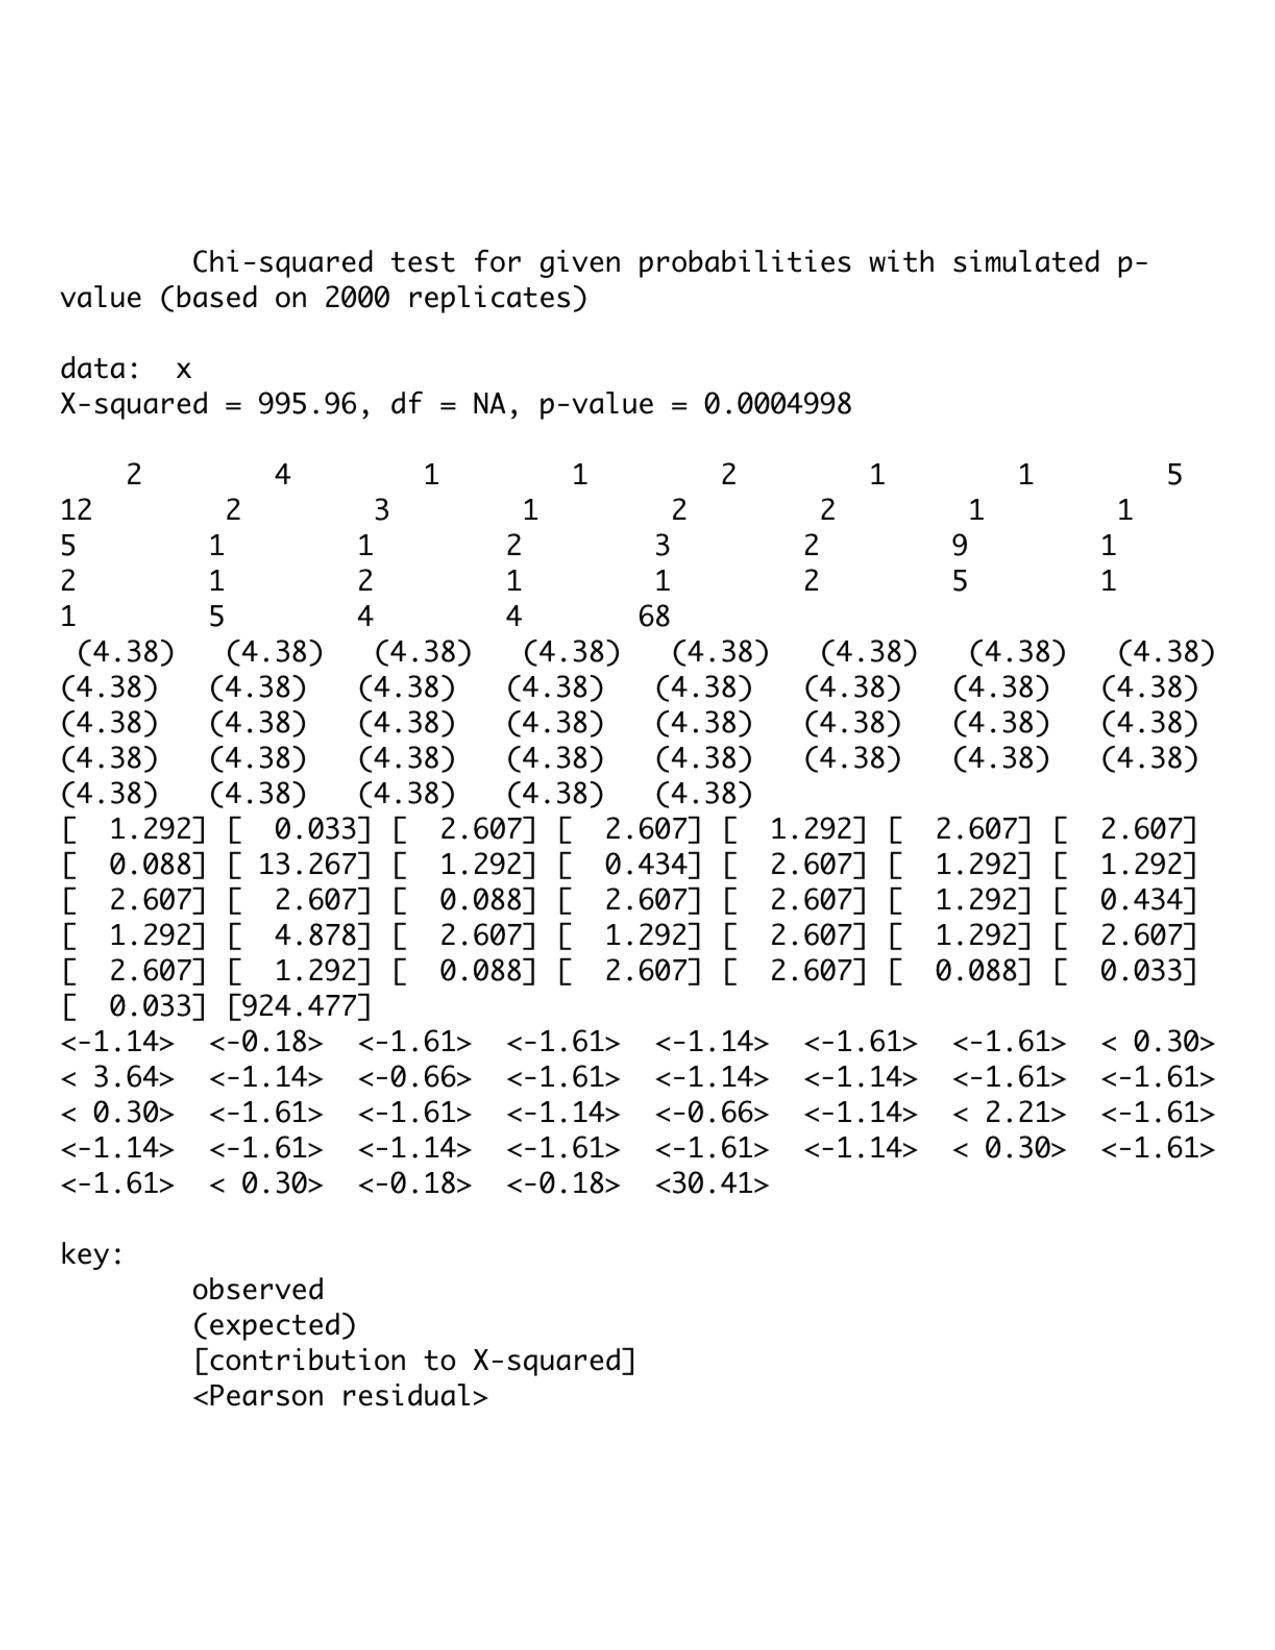
\includegraphics[width=0.10]{xchisq_country.pdf}
\caption{The xchi-square test above is analyzing whether the probability of each country in a  journal article is equal. The expected numer of journal articles for each country is approximately 4. The expected values are in parentheses and the observed values are just above it.}
\label{fig: Chi Square for Country}
\end{center}
\end{figure}

From the figure above, the expected number of articles from each country is approximately 4. Yet from the observed frequencies above, we can see that many countries only have 1 or two articles with work done there, but the United States has 68. Therefore, we can say that the probability of each country being represented in a journal article might not be the same.

Being that the size of each country varies, it would not make sense for each country to have the same likelihood of being represented in a journal article. Thus, the square mileage of each country was researched in order to better estimate the probability of each country being represented in a journal article. 

\pagebreak

\subsection{Region}
The region category exhibited if any or the amount of published articles completed their study in a particular region. This allowed us to see which region were more or less commonly seen for ecology work. The following contingency table counts the number of times a region was represented in the data set.
\begin{table}[h]
\begin{center}
\begin{tabular}{|c|c|}
\textbf{Region} & \textbf{Count}\\
$East-North Central$ & 7\\
$Mid-Atlantic$ &  3\\
$Mountain$ &  12\\
$New England$ & 3\\
$North West$ & 3\\
$Pacific$ & 24\\
$South Atlantic$ & 10\\
$West North Central$ & 3\\
$West South Central$ & 3\\
\end{tabular}
\end{center}
\caption{This is the contingency table for the regions. It shows the number of journal articles that had work done on each region.}
\label{fig: Region Contingency Table}
\end{table}
From the table above notice the number of published articles is higher in the Pacific region in comparison to the other regions.

If there is an assumption that the probability of each region being represented in a journal entry is the same, then there should be the same number of counts for each region. Below, is a XChi-Square test that shows if this statement is true or not. 

\begin{figure}[h]
\begin{center}
\includegraphics[width=0.10]{RegionsChiSquare1.pdf}
\label{fig: Region XChi-Square}
\caption{This is the XChi-Square test on the regions.}
\end{center}
\end{figure}

From the Pearson residuals notice that Pacific has the most positive residual thus, the observed frequency exceeds the expected frequency. Additionally, Mid-South and North West has the most negative residual thus, the observed frequency does not meet the expected frequency. Through visual representation, figure *#* clarifies this idea. The pie chart on the left shows what the pie chart should look like if every region had an equal chance of being represented in a published article. While the pie chart on the right is what the pie chart looks like when using the counts from the data set. 

\begin{figure}[h]
\begin{center}
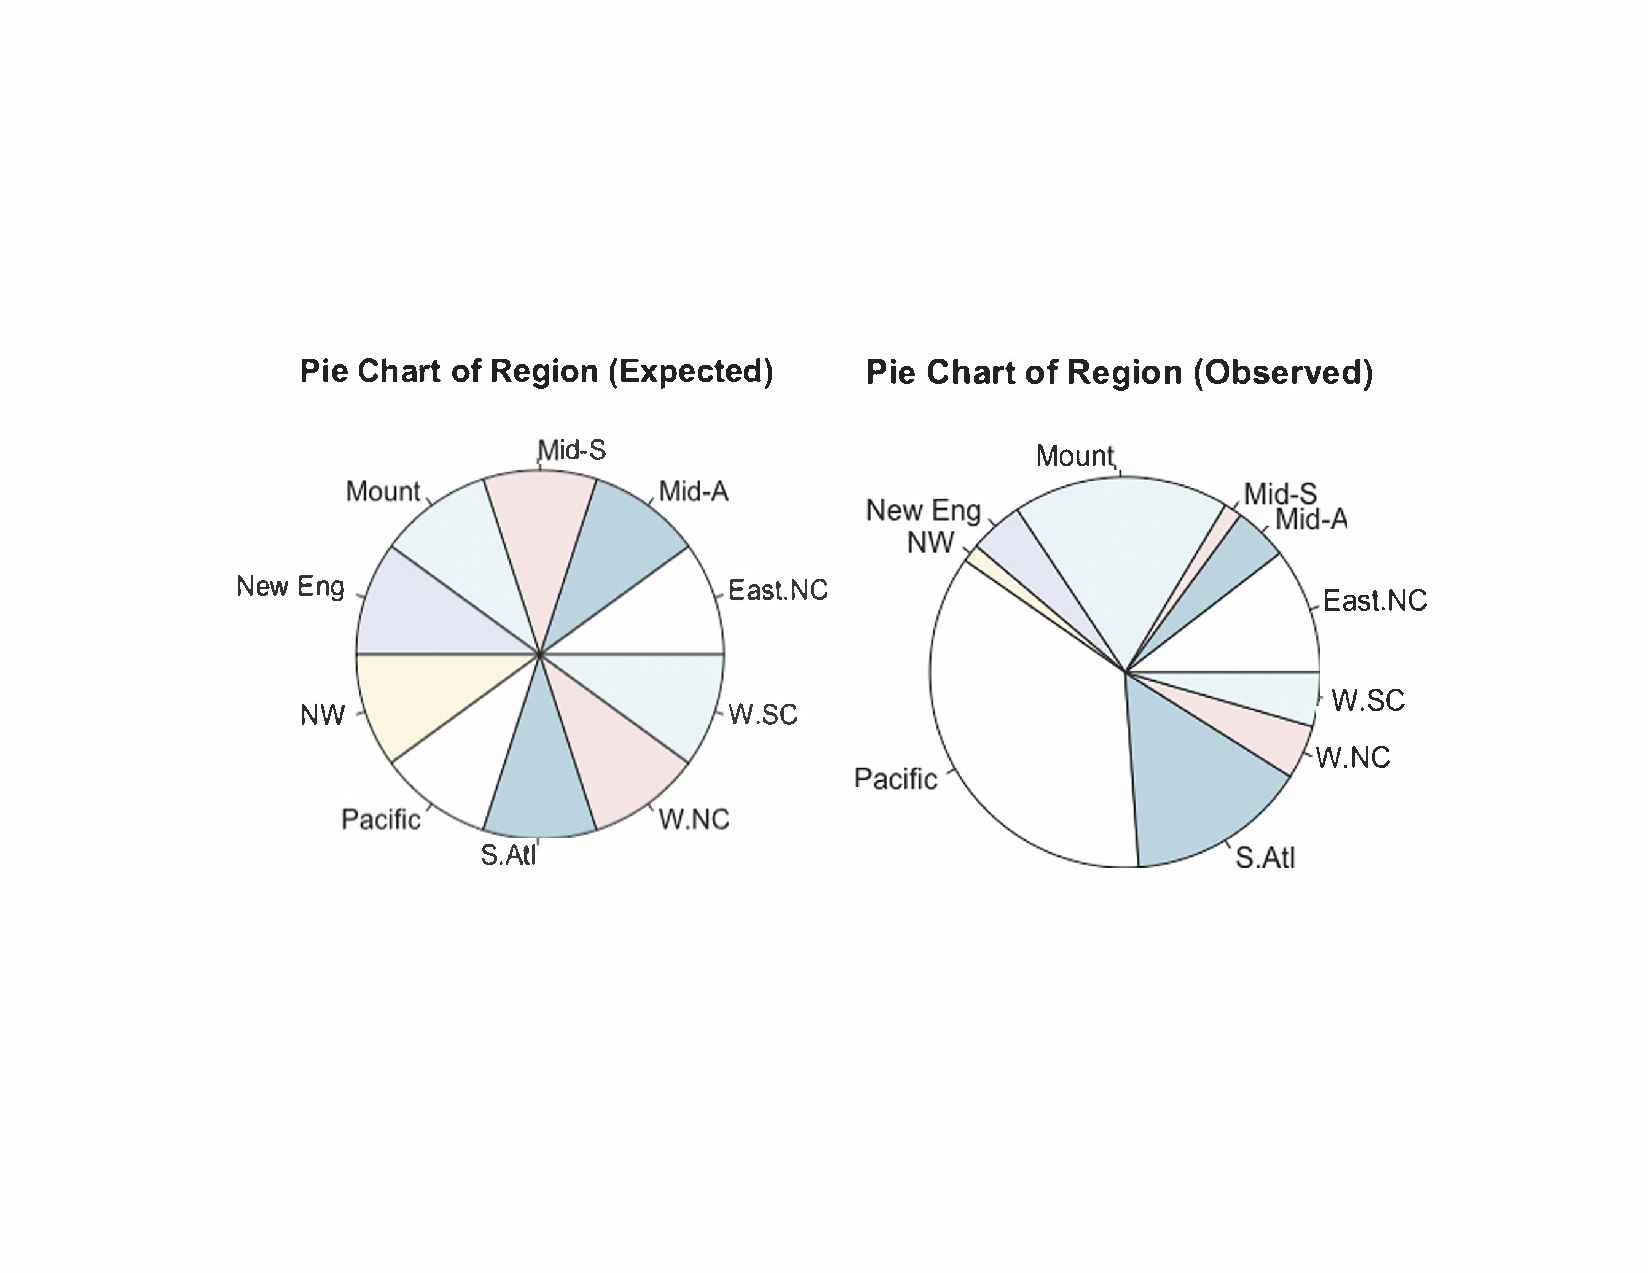
\includegraphics[width=0.10]{RegionsPieChart.pdf}
\label{fig: Region Pie Chart}
\caption{The pie charts above depict the expected and observed number of journal entries in each region.}
\end{center}
\end{figure}

**Missing pic in github**

If the regions had a equal chance of being represented in these published articles these pie charts would look similar. Unfortunately, this is not the case and it is obvious that Pacific takes up the majority of the pie chart.

If there is an assumption that the probability of each region being represented in a journal entry is the same as each region's square mileage/ Then the region with a larger square mileage would have more published articles than those regions with a smaller square mileage. Below, is a Chi-Square test that shows if this statement is true or not.

\begin{figure}[h]
\begin{center}
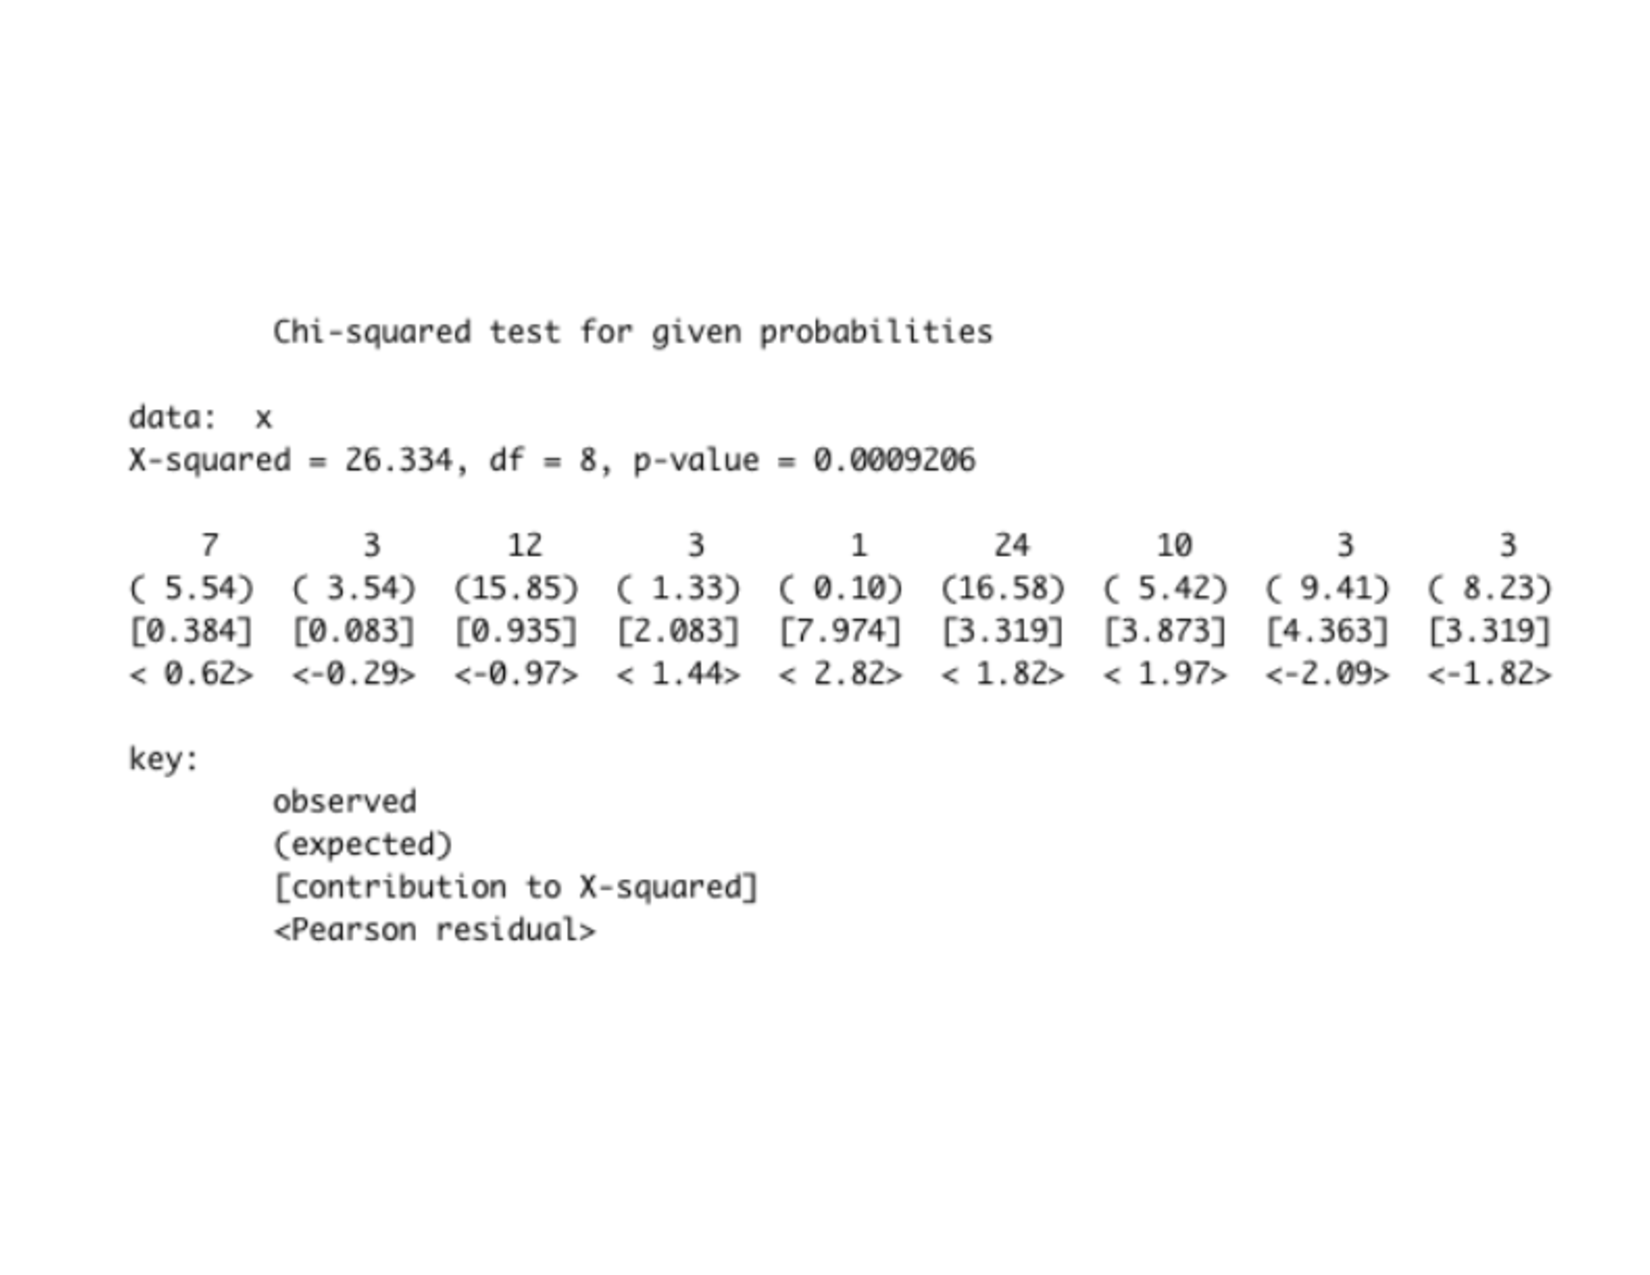
\includegraphics[width=10cm]{RegionChiSquare2.pdf}
\label{fig: Region XChi-Square with Square Mileage}
\caption{This is XChi-Square test on region, using square mileage in order to create expected values.}
\end{center}
\end{figure}

Looking into the Pearson residuals notice that North West has the most positive residual thus showing that the observed frequency exceeds the expected frequency. Through visual representation, figure *#* clarifies this idea. The bar graph on the left is the number of journals one expects to see given each region's square mileage. The bar graph on the right is what was observed using the counts from the data set. Also, due to unidentifiable region we couldn't locate square mileage for Mid-South. Due to this, we redid some data cleaning to remove this region. So our results do not include this specific region.

\begin{figure}[h]
\begin{center}
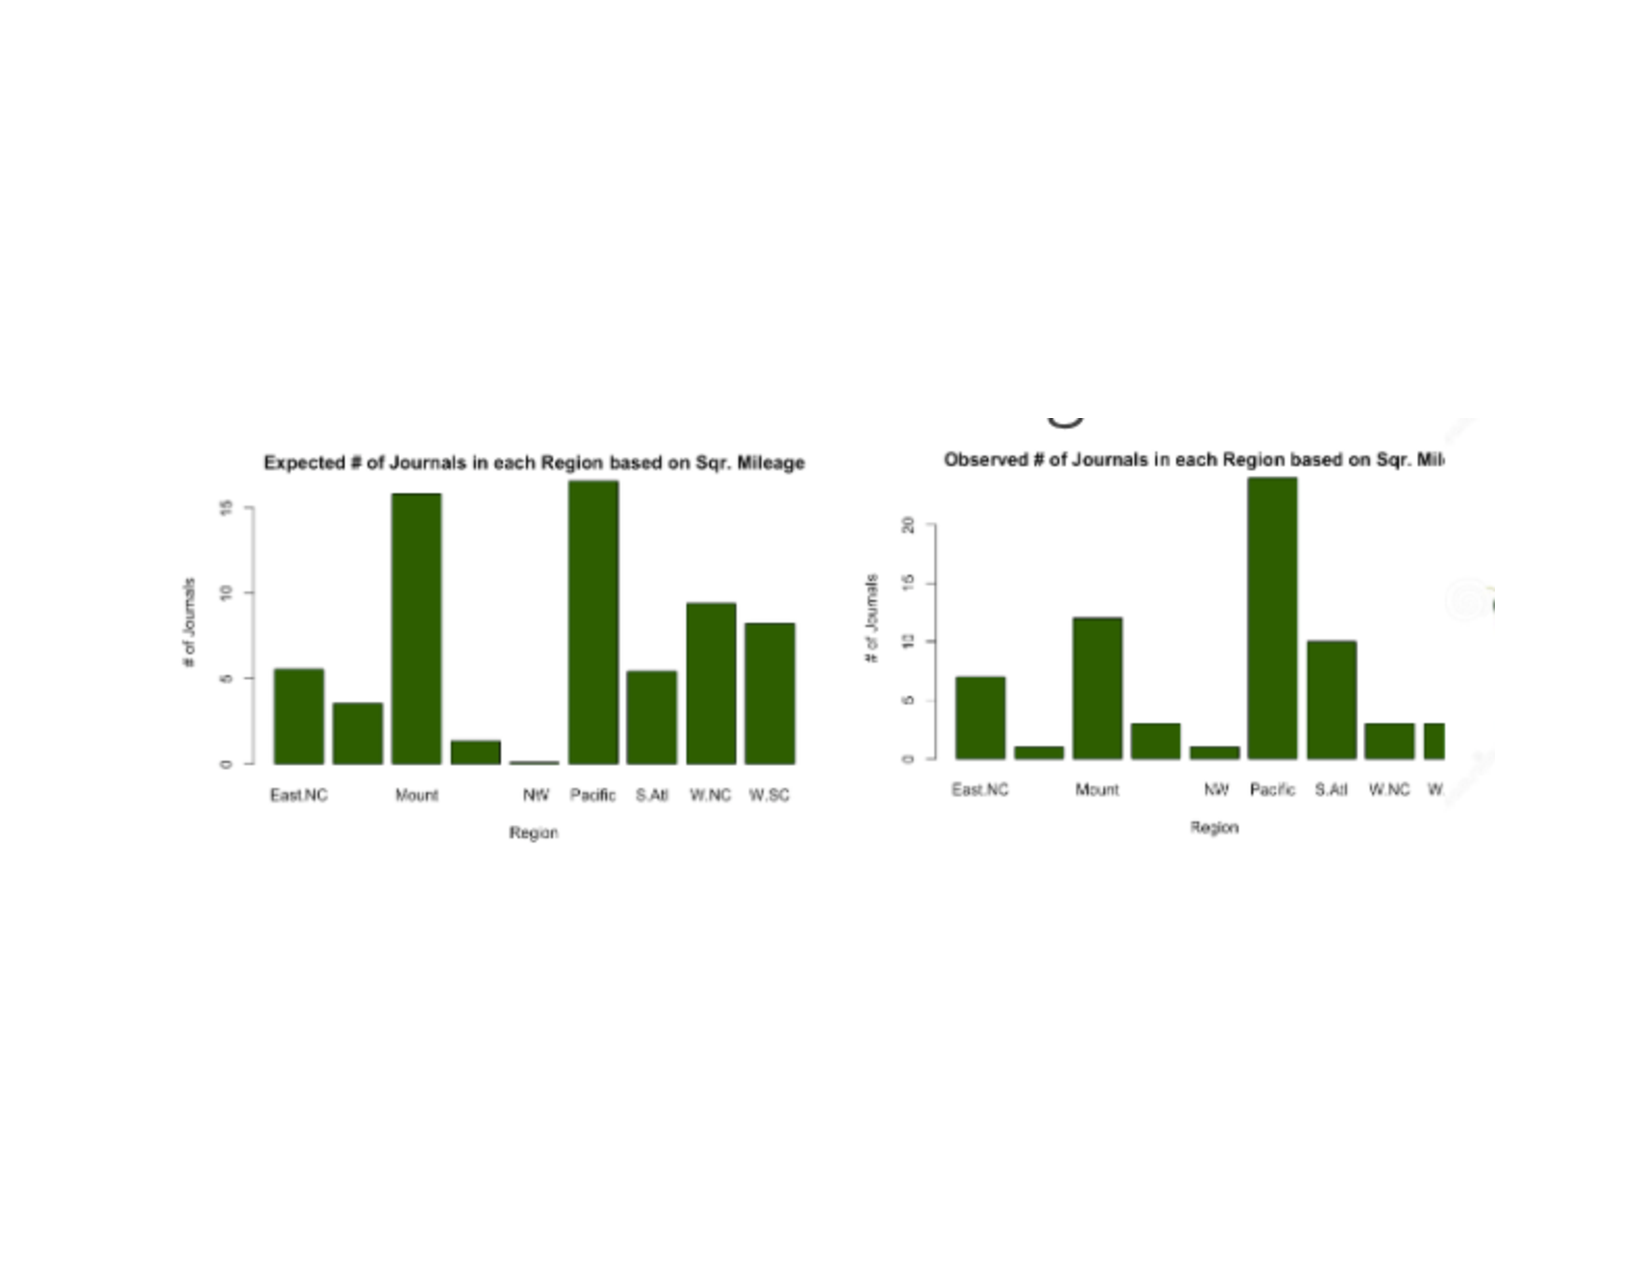
\includegraphics[width=10cm]{Regions2BarGraph.pdf}
\label{fig: Continent Bar Graph}
\caption{The bar graph above depicts the expected and observed number of journal entries in each region.}
\end{center}
\end{figure}


\pagebreak

\subsection{State}
The state category noted if and how many of these published articles completed their study in a particular state. This allowed us to see which states were more or less popular for ecology work. The following contingency table counts the number of times a state was represented in the data set. 
\begin{table}[h]
\begin{center}
\begin{tabular}{|c|c|}
\textbf{State} & \textbf{Count}\\
$AK$ & 2\\
$AL$ &  2\\
$AZ$ &  3\\
$CA$ & 13\\
$CO$ & 2\\
$FL$ & 4\\
$HI$ & 1\\
$IN$ & 1\\
$KS$ & 2\\
$MA$ & 1\\
$MD$ &  1\\
$MI$ &  4\\
$MO$ & 1\\
$MT$ & 1\\
$NC$ & 1\\
$NH$ & 1\\
$NJ$ & 2\\
$NM$ & 1\\
$NY$ & 1\\
$OH$ &  1\\
$OR$ &  4\\
$TX$ & 3\\
$UT$ & 1\\
$WA$ & 3\\
$WI$ & 1\\
$WY$ & 2\\
\end{tabular}
\end{center}
\label{fig: State Contingency Table}
\caption{The above table shows the number of journal articles that had research done in each state.}
\end{table}

From the table above, one can tell that most of the journal entries are published when the work was in California. The states that are not included in the table were never represented in the data set. 
If there is an assumption that the probability of each state being represented in a journal entry is the same as each state's square mileage then the larger states would have more published articles than the smaller states. Below, is the Chi-Square test that test if this statement is true. 

\begin{figure}[h]
\begin{center}
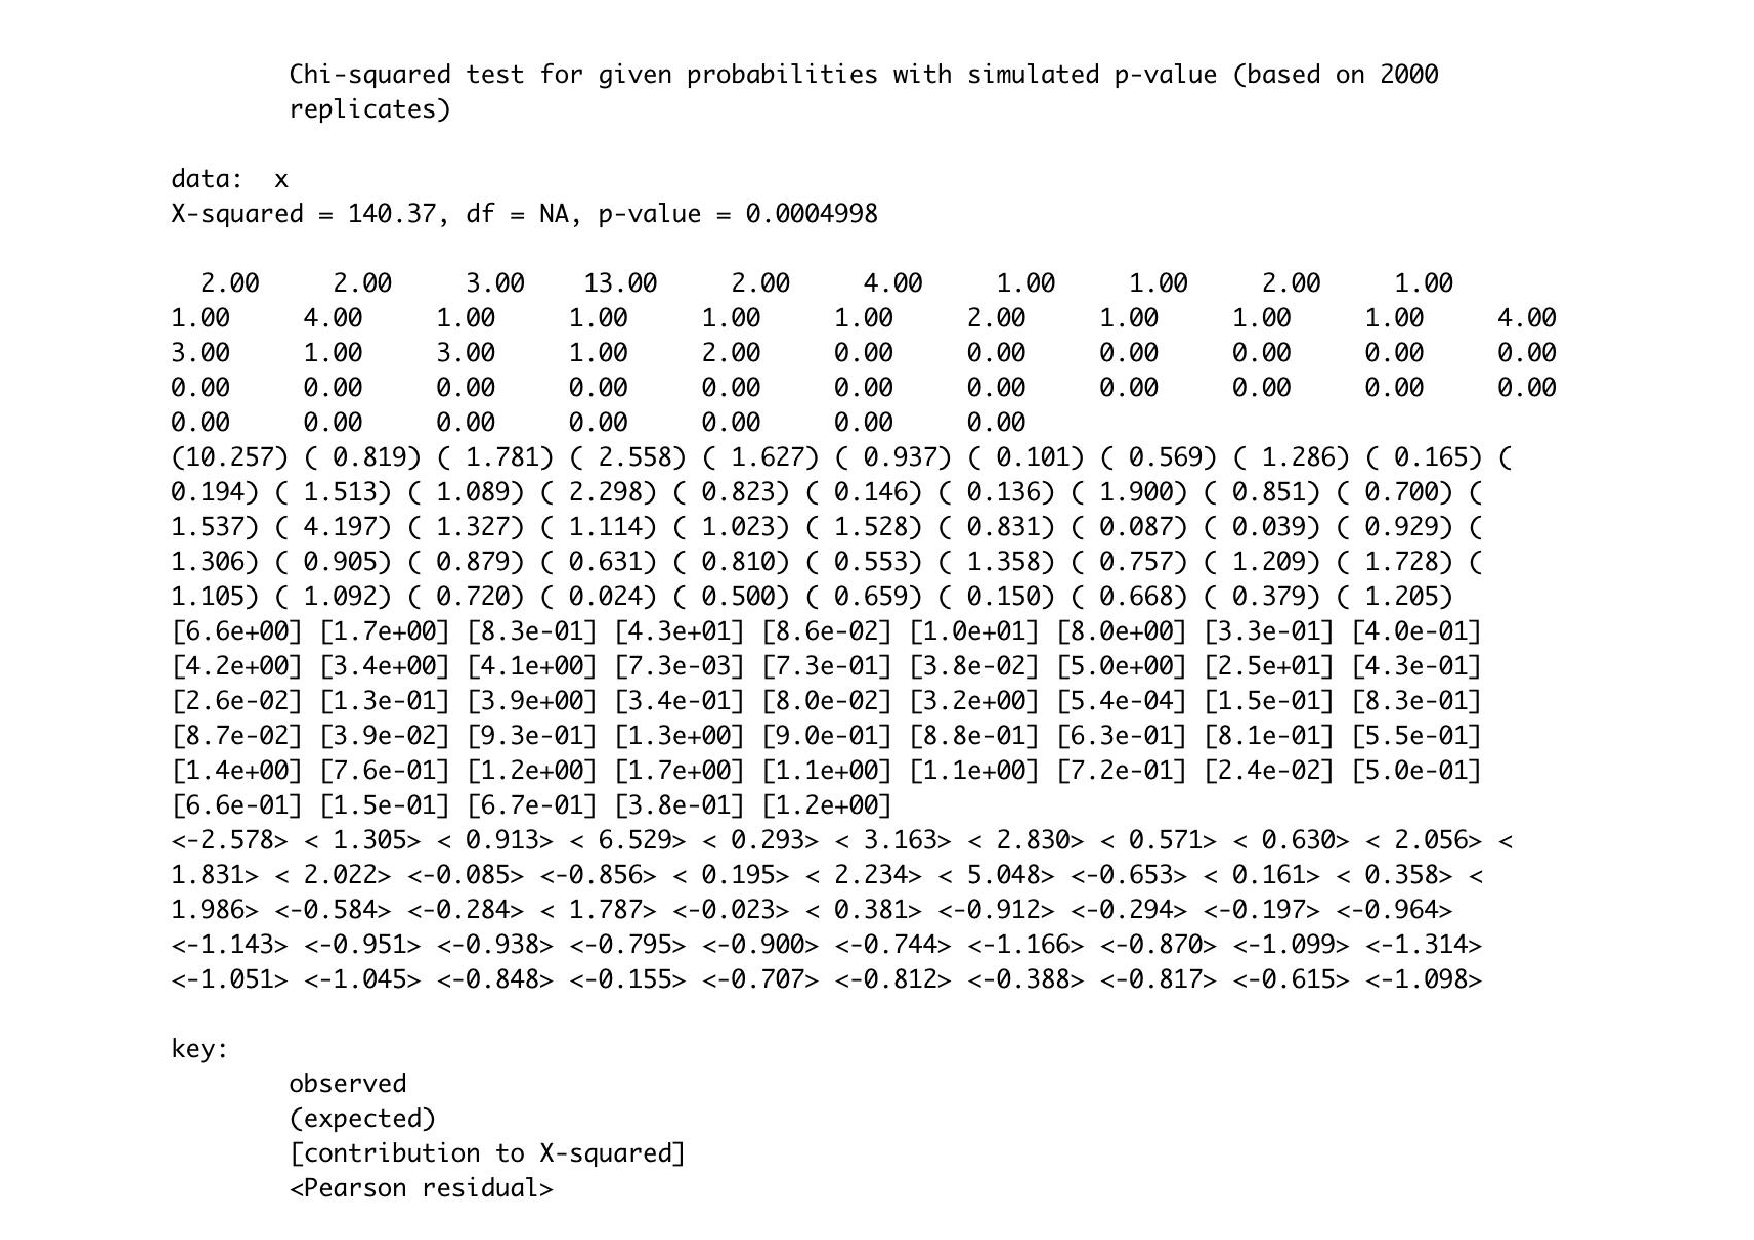
\includegraphics[width=10cm]{chi-state.pdf}
\label{fig: Chi-Square Test: States}
\caption{This is the chi-square test on the states, using square mileage to predict expected.}
\end{center}
\end{figure}

From the Pearson residuals one can note that California has the most positive residual thus, the observed frequency exceeds the expected frequency. For a visual presentation, figure *3* helps explain this idea. The map on the left is what the map is expected to look like based off of how large and small each state is. The map on the right is what the map looks like when using the counts from the data set. 

\begin{figure}[h]
	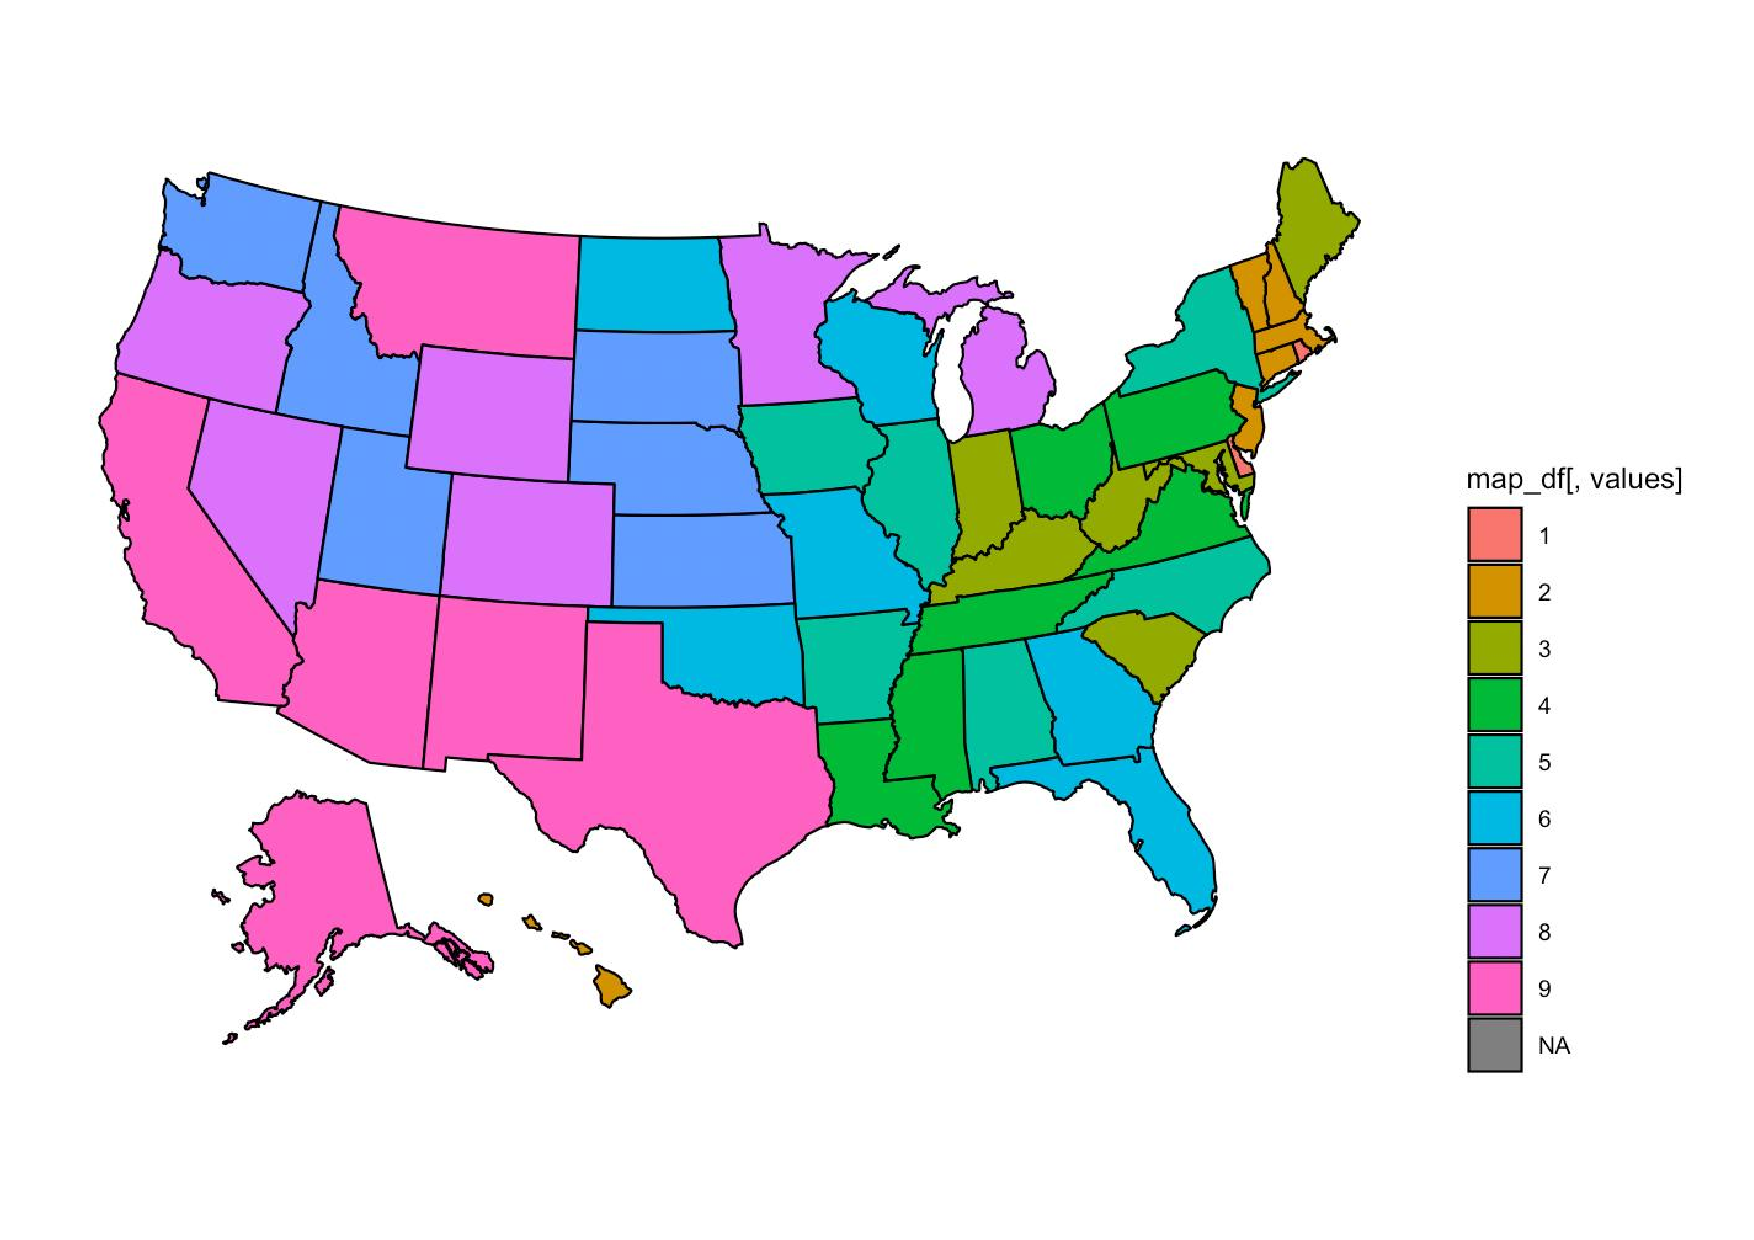
\includegraphics[width=7cm]{maps.pdf}
	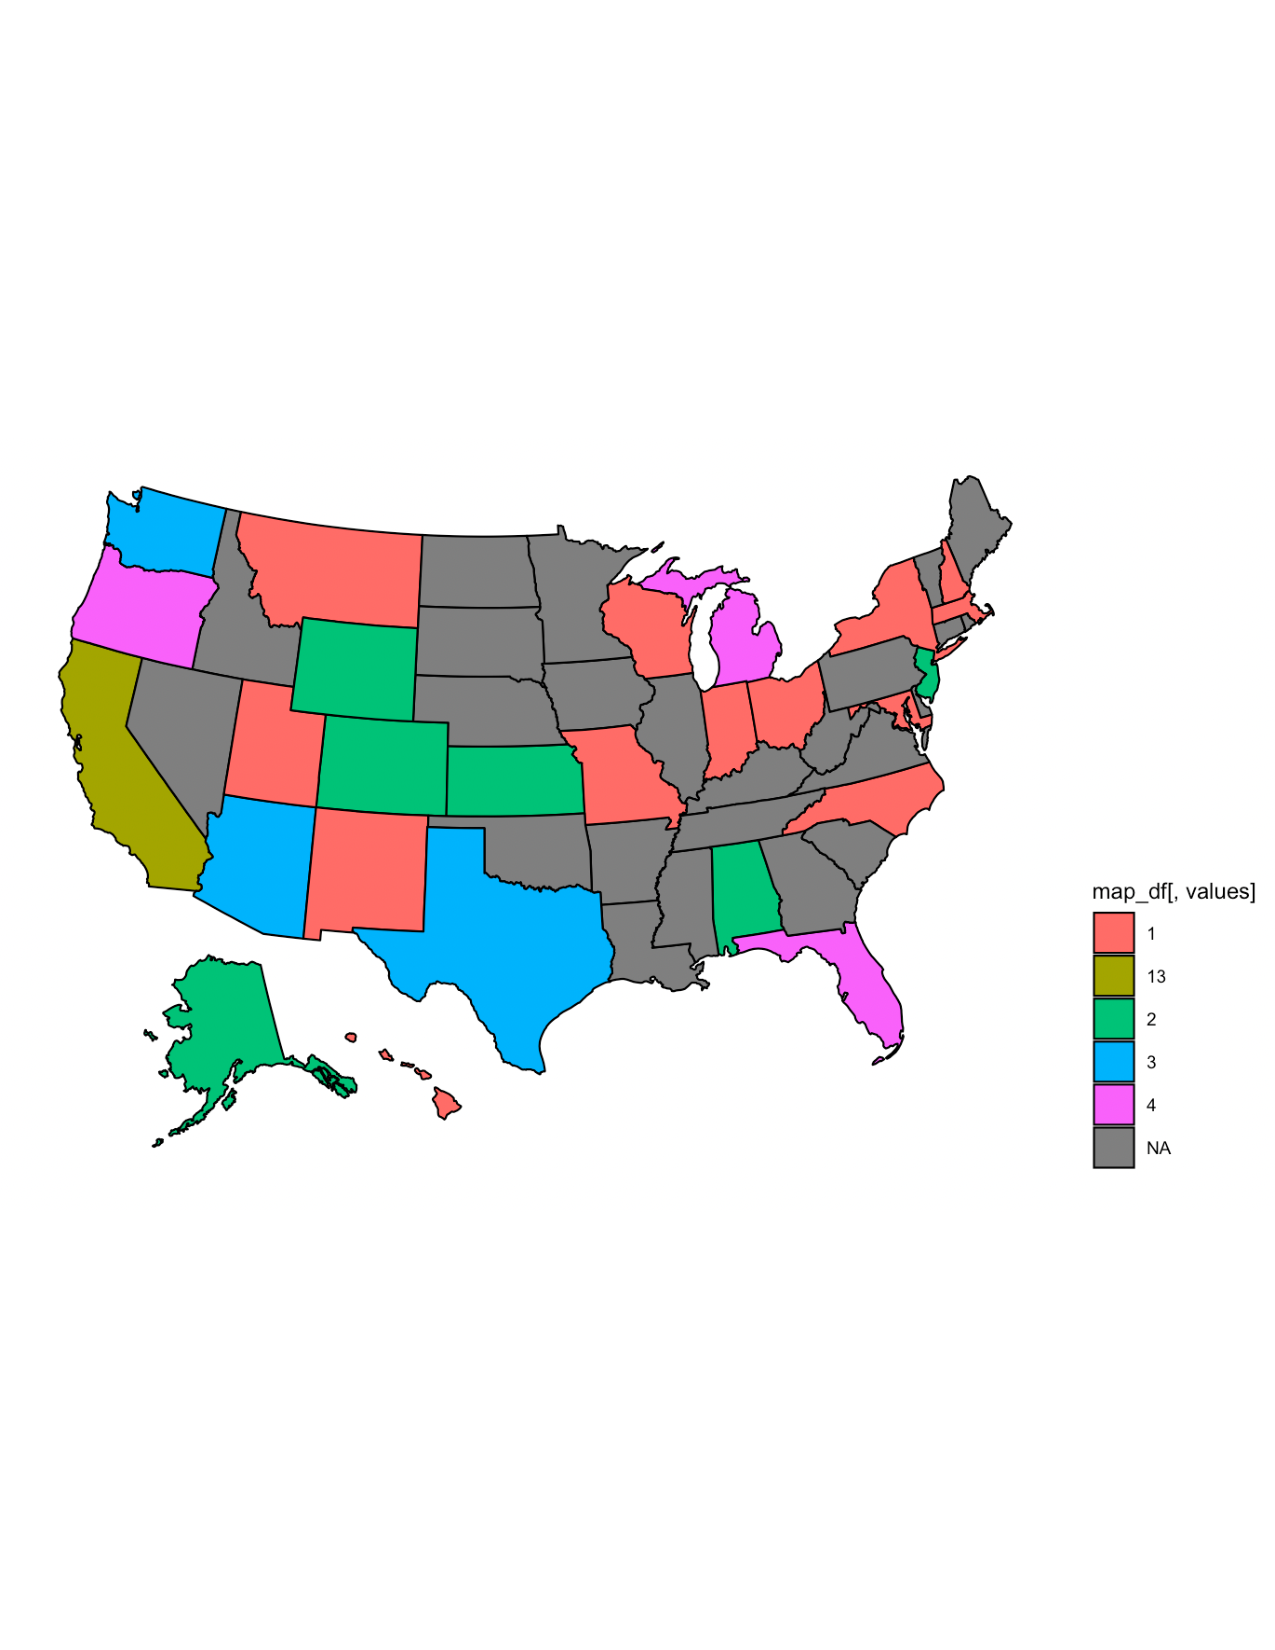
\includegraphics[width=7cm]{observed-map.pdf}
	\label{fig: Expected Frequency based on Square Mileage vs Observed Frequency}
	\caption{The charts above depict the expected and observed number of journal entries in each state.}
\end{figure}

California is a large state and the majority of the published articles had work done in California. However, all the other states do not meet the assumption. The gray states represent the sates that were never counted in the data set. From the maps, one can conclude that the probability of each state being represented in a journal entry is not the same as the states square mileage. In other words, just because a state is bigger does not mean there are more published articles from that particular state.

\pagebreak

\subsection{Ecosystem}
The ecosystem variable noted how many of the published articles used a particular ecosystem. Ecosystems were broken down into 3 categories, Marine, Terrestrial, and Freshwater. When looking at ecosystems, the idea was to see if one ecosystem was counted more than a different ecosystem. The following contingency table counts the number of times an ecosystem was represented in the data set. 
\begin{table}[h]
\begin{center}
\begin{tabular}{|c|c|}
\textbf{Ecosystem} & \textbf{Count}\\
$Marrine$ & 20\\
$Terrestrial$ &  127\\
$Freshwater$ &  12\\
\end{tabular}
\end{center}
\label{fig: Ecosystem Contingency Table}
\caption{The contingency table above shows the number of journal entries in each ecosystem.}
\end{table}

From the table above, one can tell that most of the published articles have a terrestrial ecosystem. 
If there is an assumption that the probability of each ecosystem being represented in a journal entry is the same, then there should be the same number of counts for each ecosystem. Below, is the Chi-Square test that test if this statement is true. 

\begin{figure}[h]
\begin{center}
	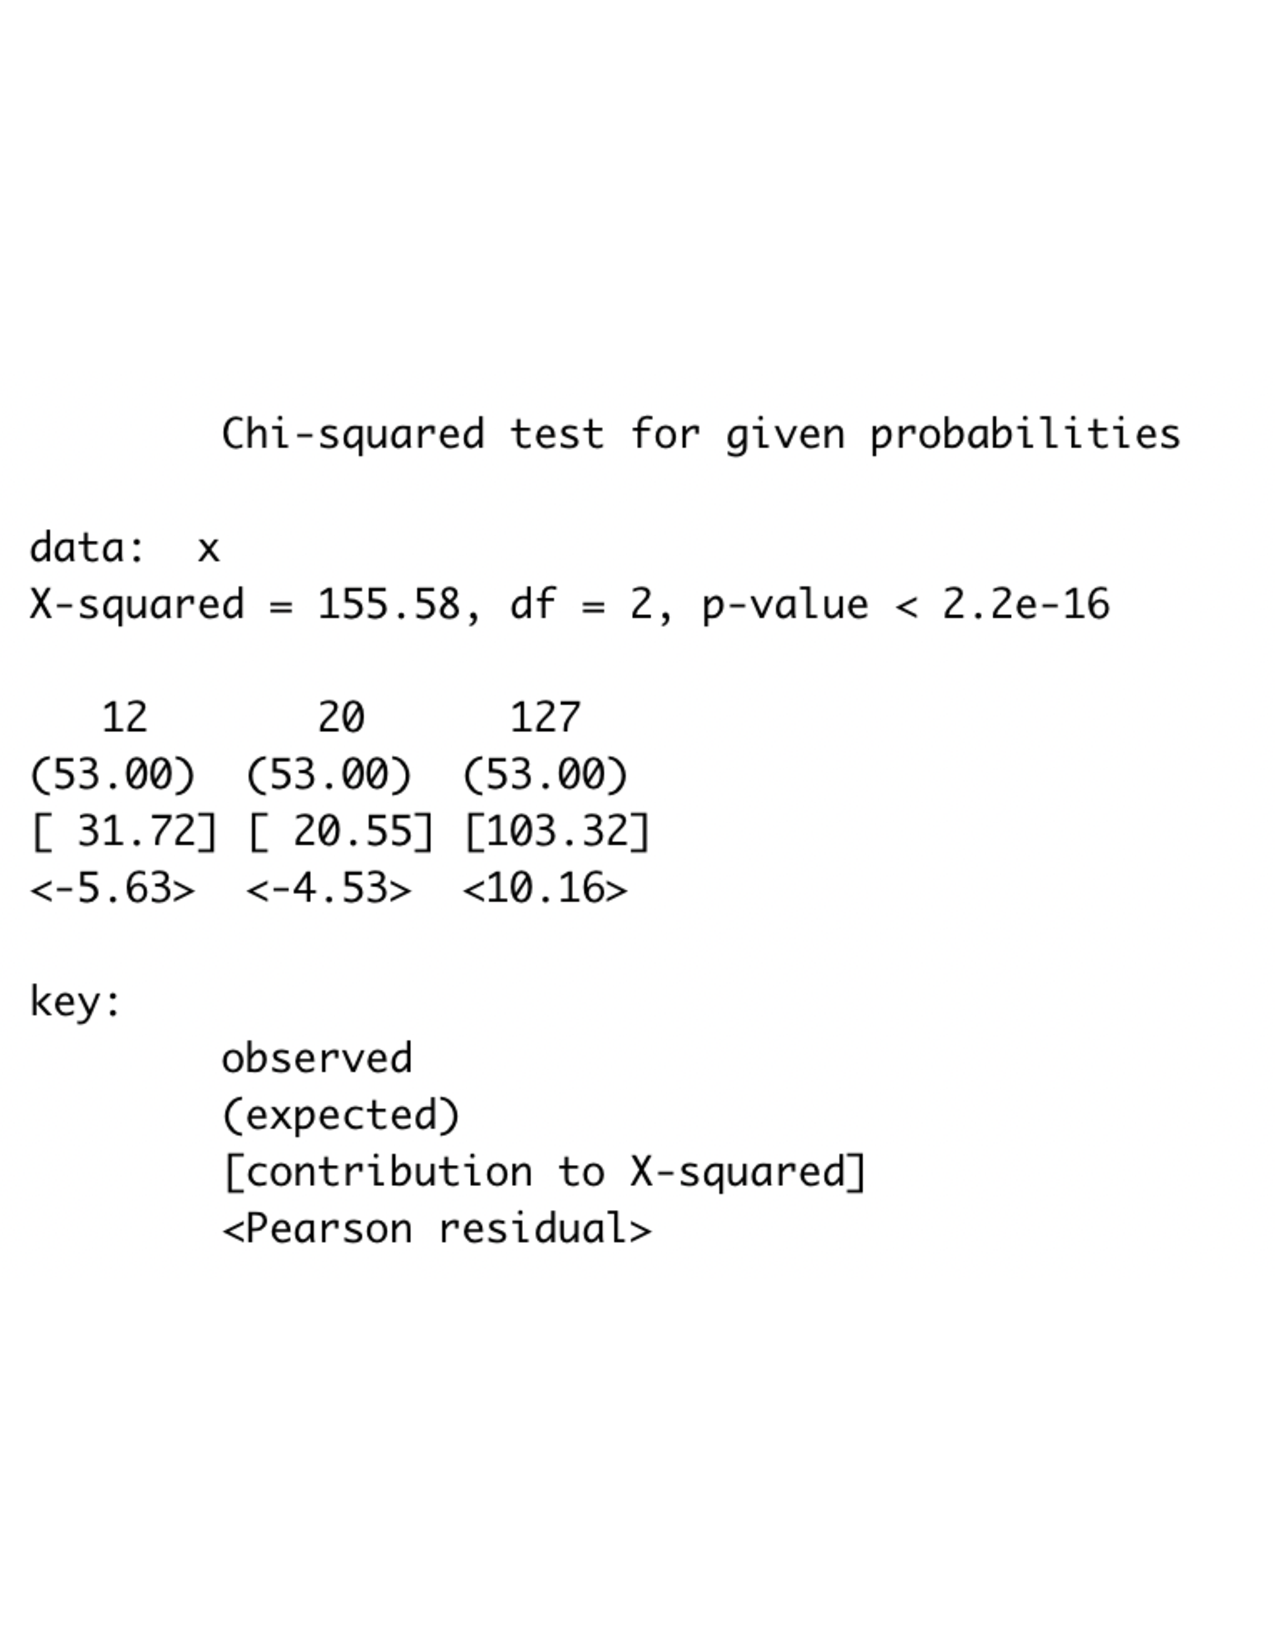
\includegraphics[width=10cm]{chi-eco-1.pdf}
	\label{fig: Chi-Square Test: Ecosystem}
	\caption{The chi-square test is looking for a difference between expected and actual values for ecosystem.}
\end{center}
\end{figure}

From the Pearson residuals one can note that terrestrial has the most positive residual thus, the observed frequency exceeds the expected frequency. Additionally,freshwater has the most negative residual thus, the observed frequency does not meet the expected frequency. For a visual presentation, figure *3* helps explain this idea. The pie chart on the left shows what the pie chart should look like if every ecosystem had an equal chance of being represented in a published article. While the pie chart on the right is what the pie chart looks like when using the counts from the data set. 

\begin{figure}[h]
\begin{center}
	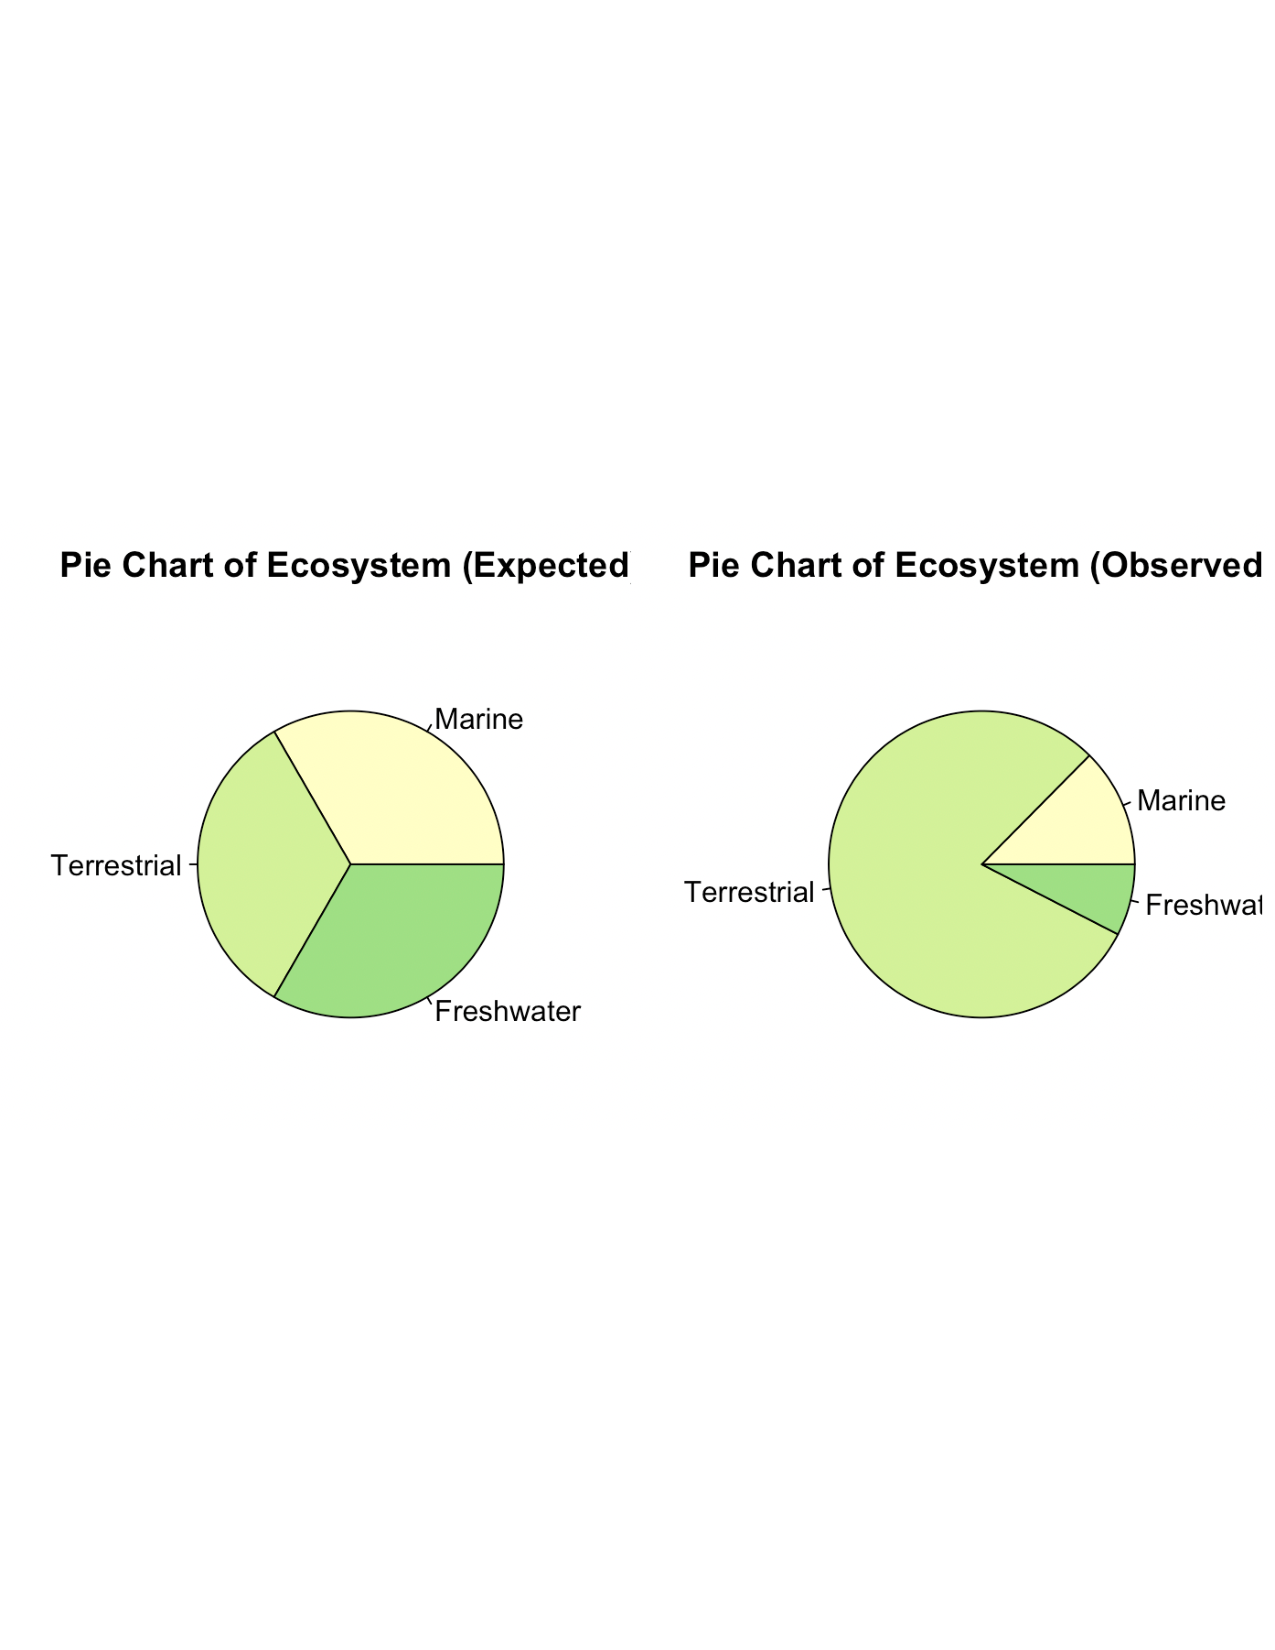
\includegraphics[width=10cm]{pie-eco-1.pdf}
	\label{fig: Expected Frequency vs Observed Frequency}
	\caption{The pie charts above depict the expected and observed number of journal entries in each ecosystem.}
\end{center}
\end{figure}
If the ecosystems 
had a equal chance of being represented in these published articles these pie charts would look similar. However this is not the case and it is obvious that terrestrial takes up the majority of the pie chart. 

If there is an assumption that the probability of each ecosystem being represented in a journal entry is the same as each ecosystem's square mileage then the larger ecosystem's would have more published articles than the smaller ecosystems. Below, is the Chi-Square test that test if this statement is true. 

\begin{figure}[h]
\begin{center}
	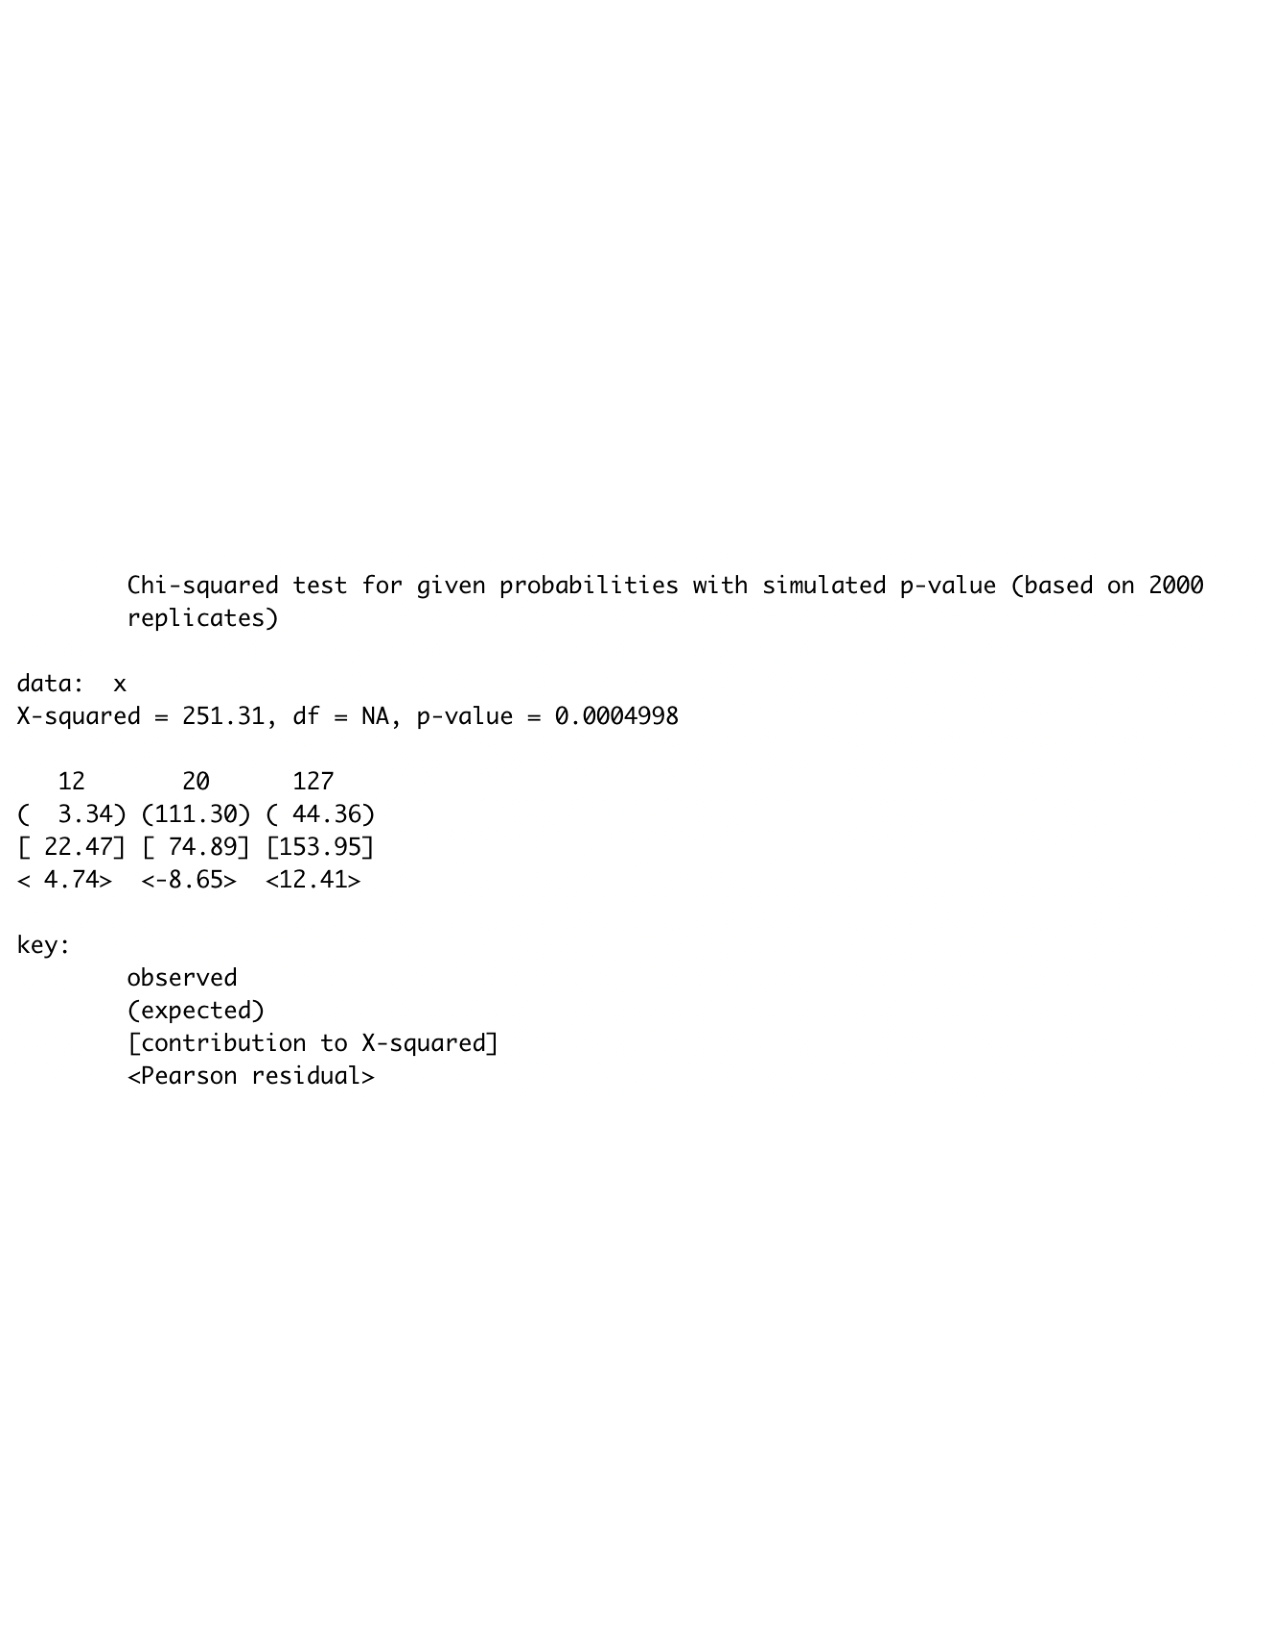
\includegraphics[width=10cm]{chi-eco-2.pdf}
	\label{fig: Chi-Square Test: Ecosystem}
	\caption{The chi-square test is looking for a difference between expected and actual values for ecosystem, while using square mileage.}
\end{center}
\end{figure}

Terrestrial has the most positive residual and marine has the most negative residual. Figure *3* shows what the expected counts should look like and what the observed counts were. 

\begin{figure}[h]
\begin{center}
	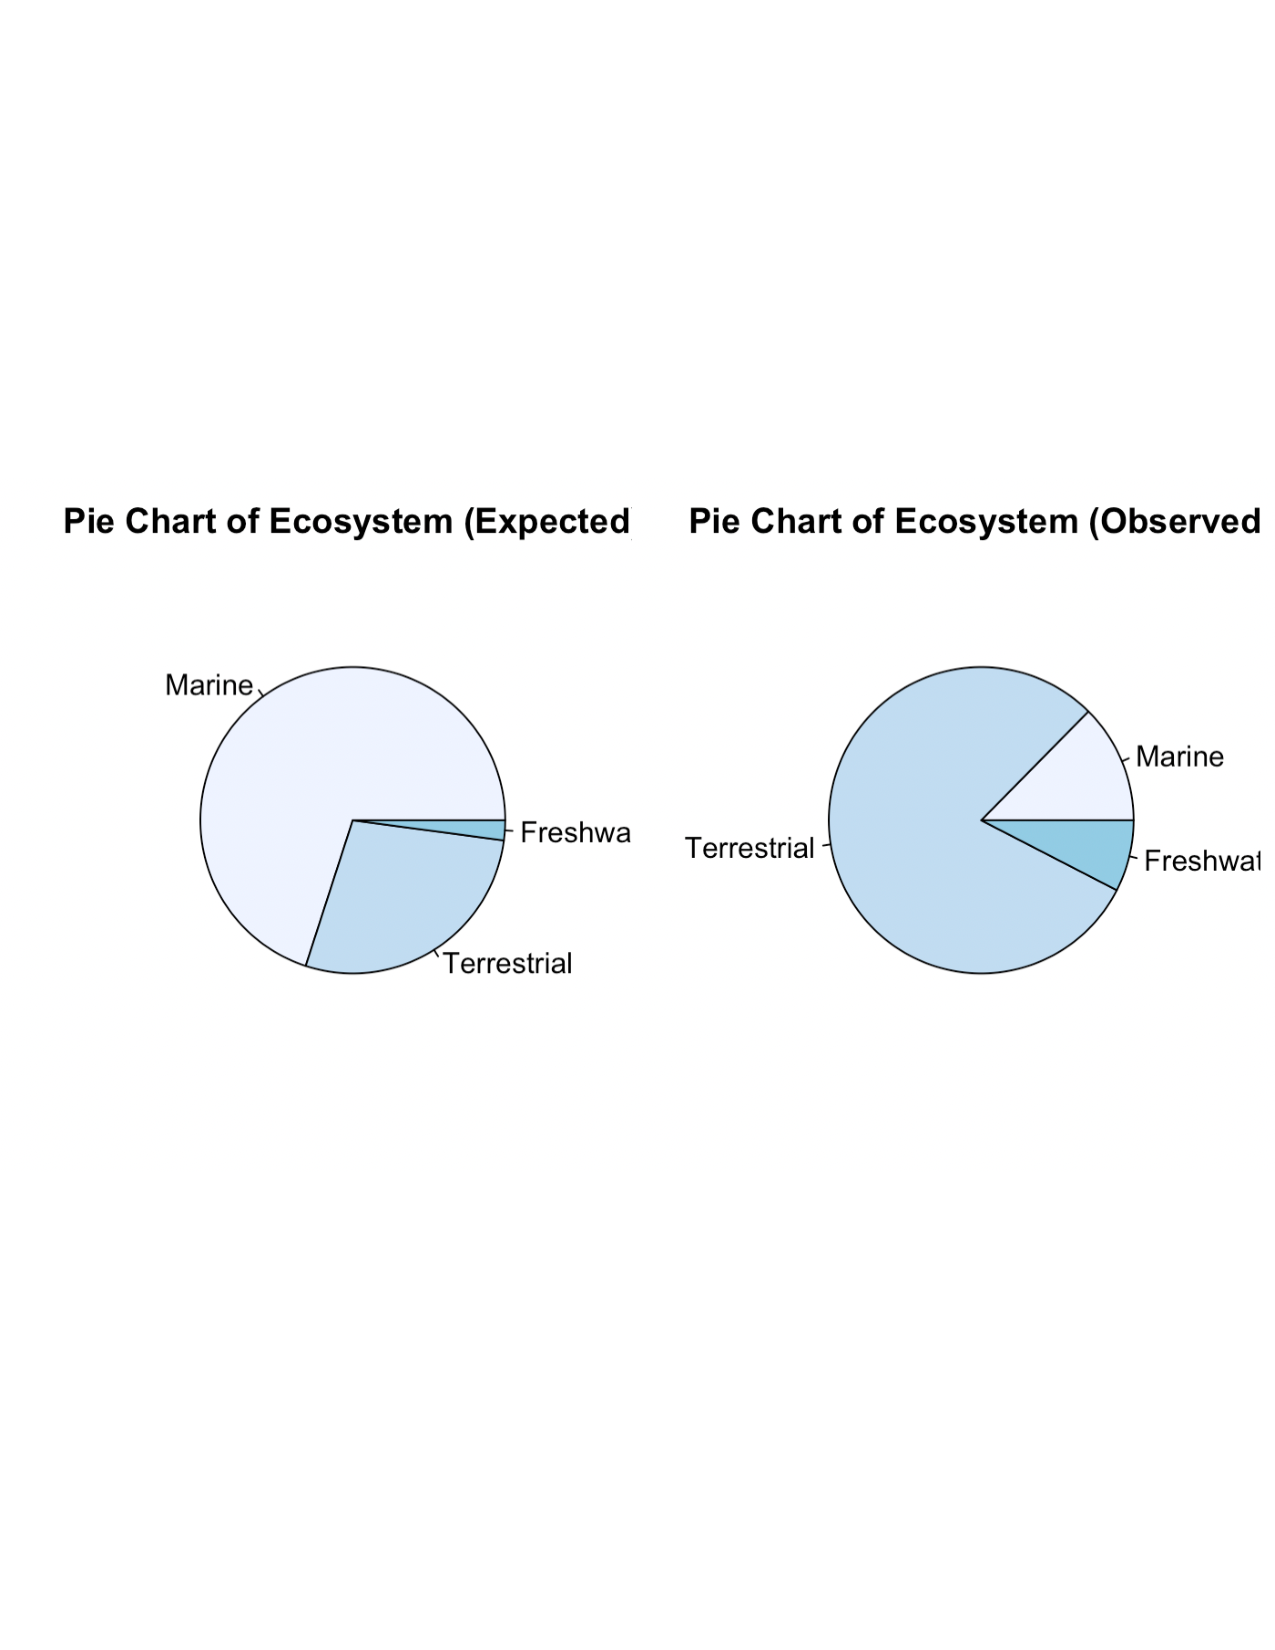
\includegraphics[width=10cm]{pie-eco-2.pdf}
	\label{fig: Expected Frequency based on Square Mileage vs Observed Frequency}
	\caption{The pie charts above shows the expected frequency based on square mileage vs the observed.}
\end{center}
\end{figure}

These bar charts do not match up thus, we cannot conclude that the probability of each ecosystem being represented in a journal entry is the same as each ecosystem's square mileage.

\pagebreak

\section{Discussion}
Due to the data not being random and there only being qualitative variables, there was not much statistical analysis to be done. For the next time the study is done, we have come up with two different ways to approach the study. If the research question was: Do publishing companies publish more articles with work done in their region, in comparison to work done outside of their region? The goal of using this question is to eliminate the need for data on journal articles that were not published. The study would focus on articles from different publishing companies, but all from the same year. The regions from which they published the most would be analyzed for any kind of bias. This would be an observational study looking at the counts of journal articles from each region. 

Another approach would be to consider published articles that have significant results. The research question is: Is there a greater percentage of published articles that have a statistically significant p-value (p < 0.05) in comparison to those who do not? The goal of using this question would also be to  eliminate the need for data on journal articles that were not published, due to the population being all published articles on ecology. This would be an observational study, that would be conducted by looking at different publishing companies from the same year and calculating the proportion of published articles that had a p-value less than 0.05. This would be the test statistic used to determine if there is any statistically significant difference in the proportion of published articles with significant p-values. 

Although both of these approaches fix the need for unattainable data, they still do not fix meeting the randomness assumption. In order to fix this, the data collectors can look for articles on a database, with the criteria of the year they are looking for, the subject they want to look into, and any other specifics they would like. After getting the results of the search, they could use a random number generator to select which articles they  will use for their study. This will correct the issue of the data not being randomly selected.

\end{document}